\documentclass{beamer}
\usepackage{hyperref}
\include{../style/cours-style.sty}

% Title
\title[LINUX2]{Linux - Avancé pour Administrateur/PowerUser - LINUX2}
\author{Christophe Brun}
\institute{Digicomp}
\date{17 avril 2024}
\beamertemplatenavigationsymbolsempty

\titlegraphic{
    \bigbreak
    
\includegraphics{image/digicomp-logo}
    \bigbreak
    Digital competence. Made of People.
    \bigbreak
}

\begin{document}

    \begin{frame}
        \transdissolve
        \titlepage
    \end{frame}


    \section{Table des matières}\label{sec:toc}

    \begin{frame}{Table des matières}
        \tableofcontents
    \end{frame}


    \section{Programme du module}\label{sec:programme-du-module}

    \begin{frame}
        \frametitle{Linux - Avancé pour Administrateur/PowerUser}
        \framesubtitle{Objectifs des 4 jours}
        \transdissolve
        \begin{columns}
            \column{0.7\textwidth}
            \begin{scriptsize}
                \begin{itemize}
                    \item Connaître l'architecture Linux
                    \item Travailler avec des commandes avancées dans le terminal
                    \item Utiliser les commandes de filtre (\lstinline{sed}, \lstinline{grep}, \lstinline{awk}, \textit{etc}.)
                    \item Gérer les utilisateurs et groupes
                    \item Définir et modifier les autorisations
                    \item Appliquer des privilèges personnalisés
                    \item Créer, gérer et exploiter des systèmes de fichiers
                    \item Créer, gérer et surveiller des processus
                    \item Connaître les services Unix
                    \item Automatiser les tâches de maintenance (\lstinline{cron}, \lstinline{at})
                    \item Installer des logiciels
                    \item Compiler des logiciels
                    \item Connaître Shell comme langage de programmation
                    \item Concevoir et écrire vos propres petits scripts Shell
                \end{itemize}
            \end{scriptsize}
            \column{0.3\textwidth}
            
\includegraphics[width=4cm]{image/IT-man-and-penguin}
        \end{columns}
    \end{frame}


    \section{Introduction}\label{sec:introduction}

    \begin{frame}
        \transdissolve
        \frametitle{Formateur sur Linux}
        \framesubtitle{Christophe Brun, conseil en développement informatique}

        \begin{columns}
            \column{0.7\textwidth}
            \begin{itemize}
                \item Développeur freelance (Python, Java, CoBOL) et data at scale.

                \item 7 ans de conseil en développement au sein d'SSII~.

                \item 7 ans de conseil en développement en indépendant, \href{https://papit.fr}{PapIT}.

                \item Passionné~!
                \bigbreak
                \begin{columns}
                    \column{0.5\textwidth}
                    \centering
                    
\includegraphics[width=3cm]{image/logo-uppa}
                    \column{0.5\textwidth}
                    \centering
                    
\includegraphics[width=3cm]{image/logo-universite-bordeaux}
                \end{columns}
            \end{itemize}
            \column{0.3\textwidth}
            \centering
            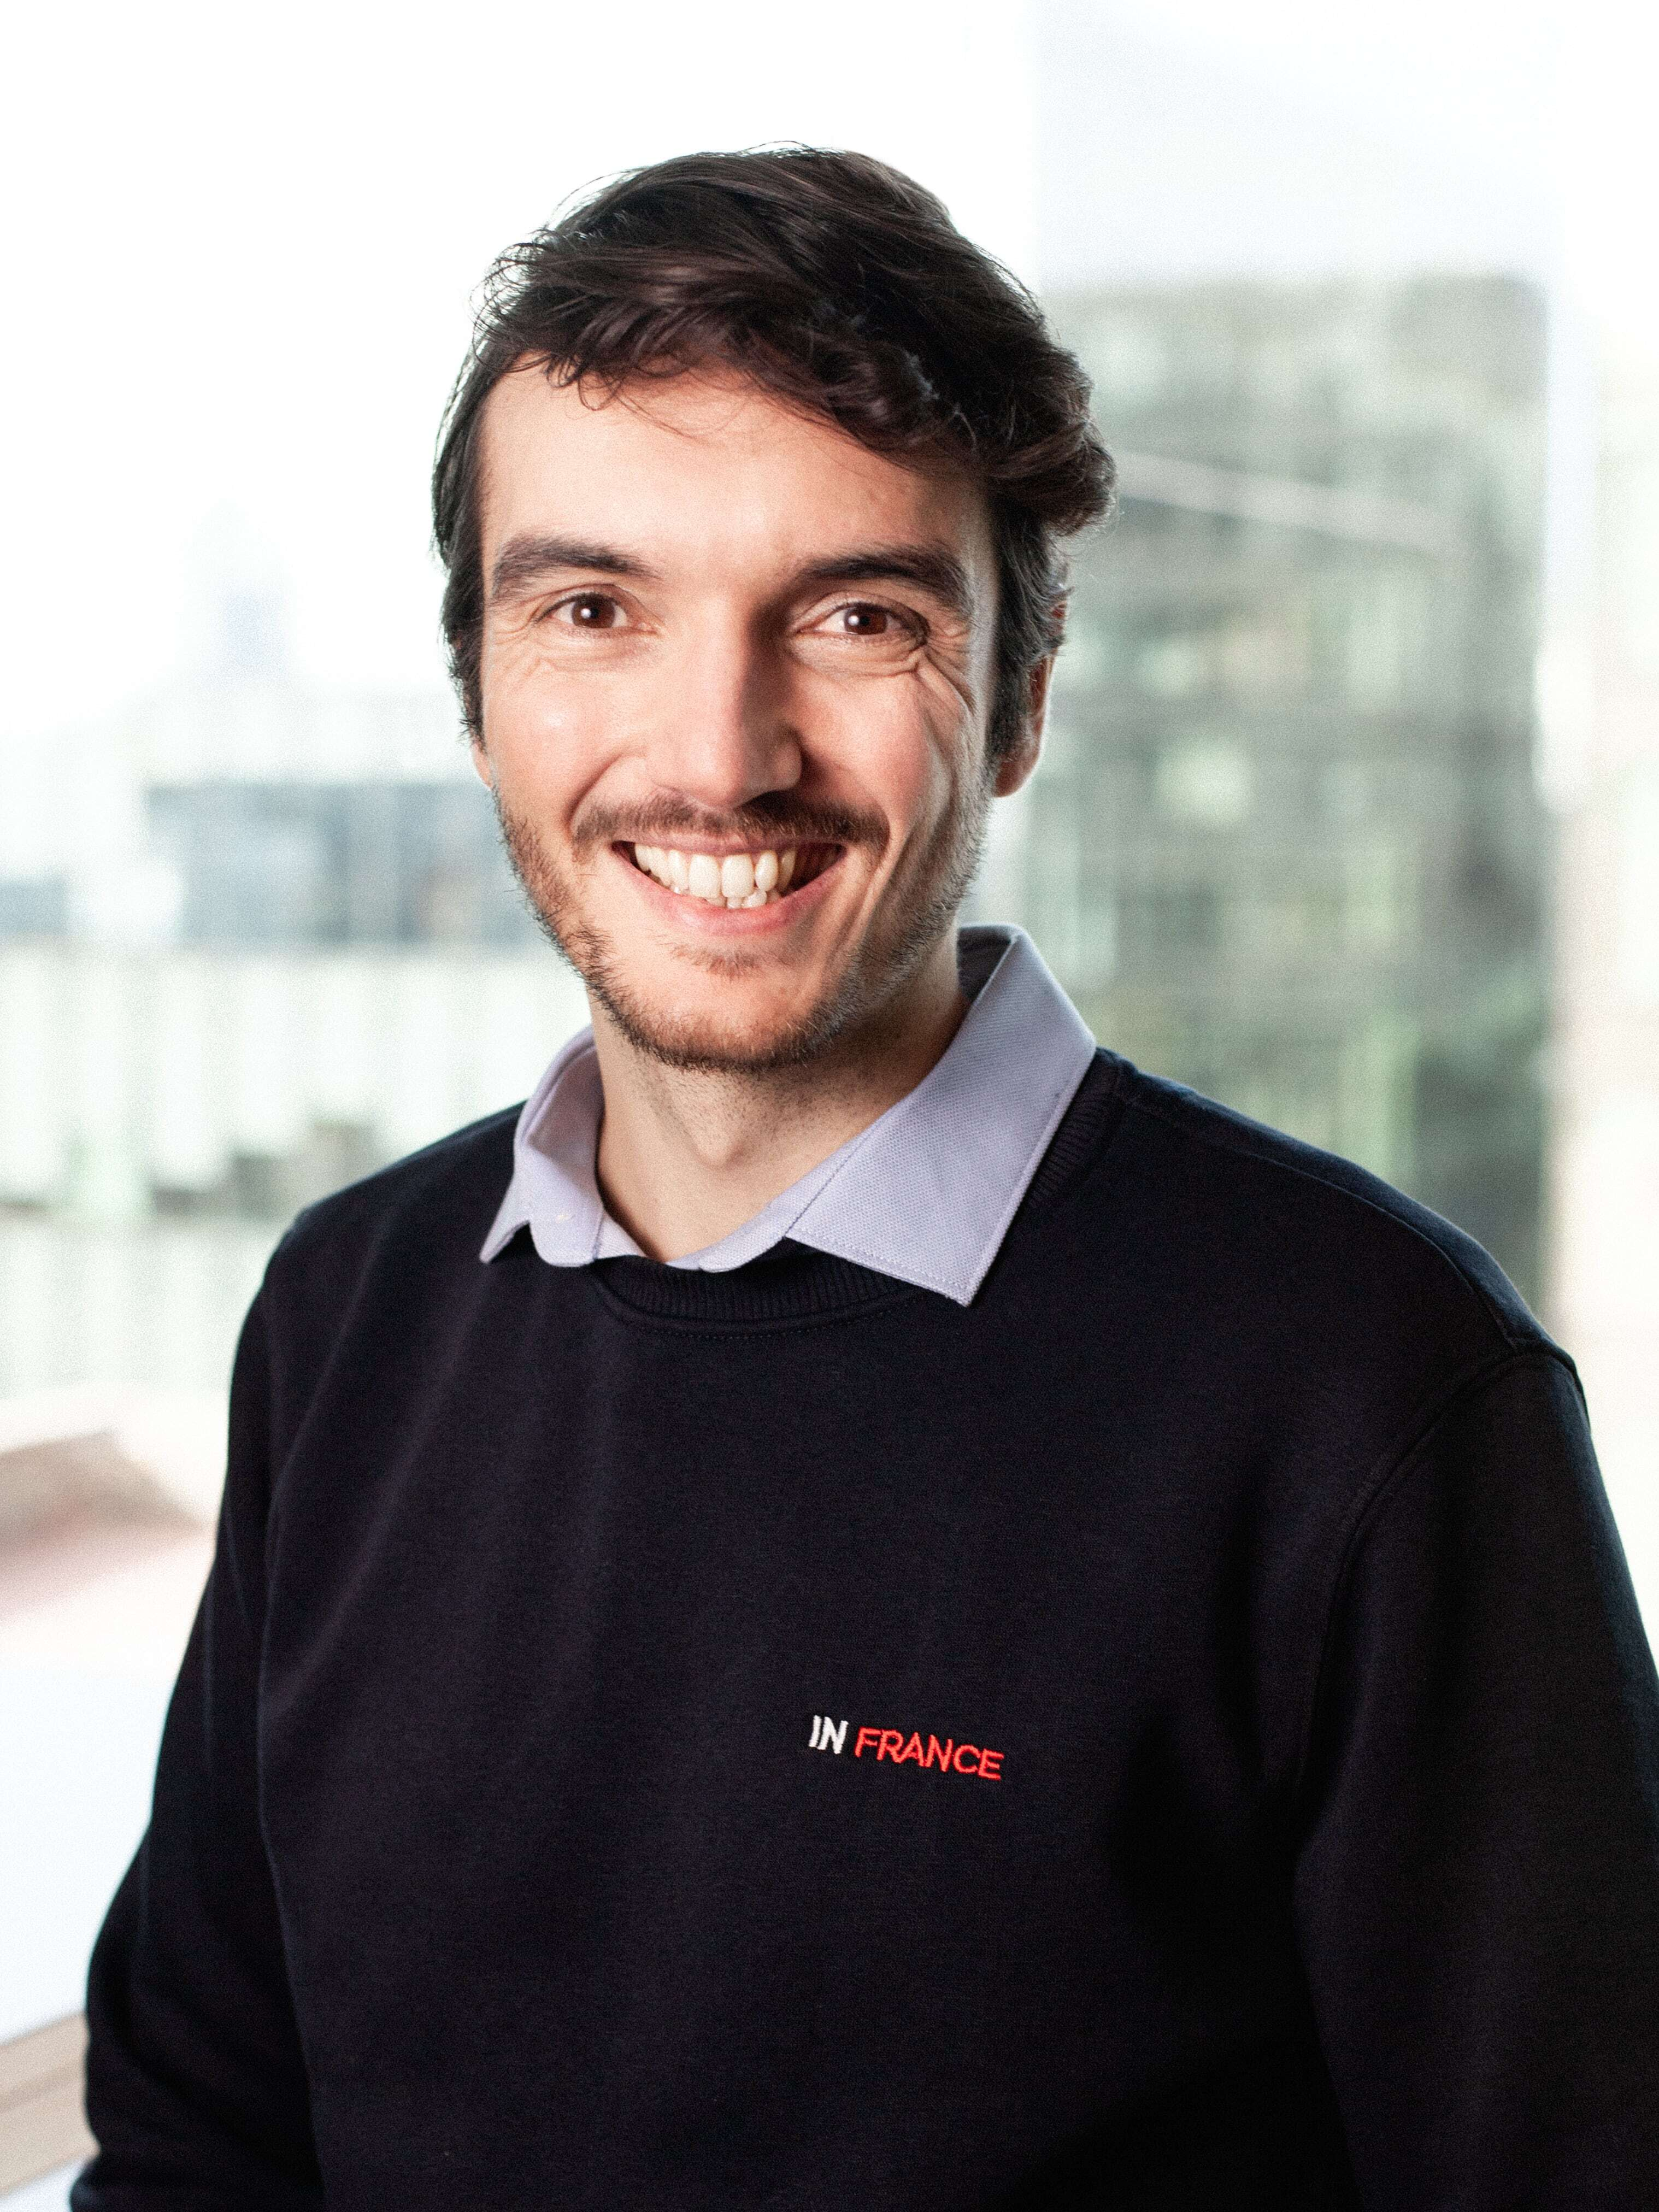
\includegraphics[width=5cm]{image/trombine-christophe}
        \end{columns}
    \end{frame}

    \subsection{Historique}\label{subsec:historique}

    \begin{frame}
        \transdissolve
        \frametitle{Historique de Linux}
        \framesubtitle{Linux, quelques caractéristiques de la première version\footnote{The early days of Linux, Lars Wirzenius, \url{https://lwn.net/Articles/928581/}}}
        \begin{footnotesize}
            \begin{itemize}
                \item La première libérée par Linus Torvald, date de 1991 et sa licence ne permet pas l'usage commercial.
                \item Compilé avec GCC 1.4, A.K.A. \textit{GNU C Compiler} de Richard Stallman.
                La publication de GCC en version 0.9 date de 1987.
                L.~Torvald a déjà porté GCC sous Minix, un OS éducatif\footnote{GCC,\url{https://gunkies.org/wiki/Gcc}}\footnotestep\footnote{A Brief Historu of GCC, \url{https://gcc.gnu.org/wiki/History}}.
                \item 1992, Linux est distribué sous license GNU GPL, donc pour tout usage, même commercial.
                \item 1992, intégration de X11, le serveur graphique, pour favoriser l'usage en \textit{desktop}.
                \item 1993, formation de la communauté Debian.
                \item Fin des années 90, les investissements d'IBM pour supporter Linux atteignent le milliard de dollars\footnote{A strong history and commitment to open source, \url{https://www.ibm.com/opensource/story/}}.
            \end{itemize}
        \end{footnotesize}
    \end{frame}

    \begin{frame}
        \transdissolve
        \frametitle{Historique de Linux}
        \framesubtitle{Historique de tous les OS\footnote{chococigar, \url{https://github.com/chococigar/cup-of-cs/blob/main/img/history\_of\_os.png}}}
        \centering
        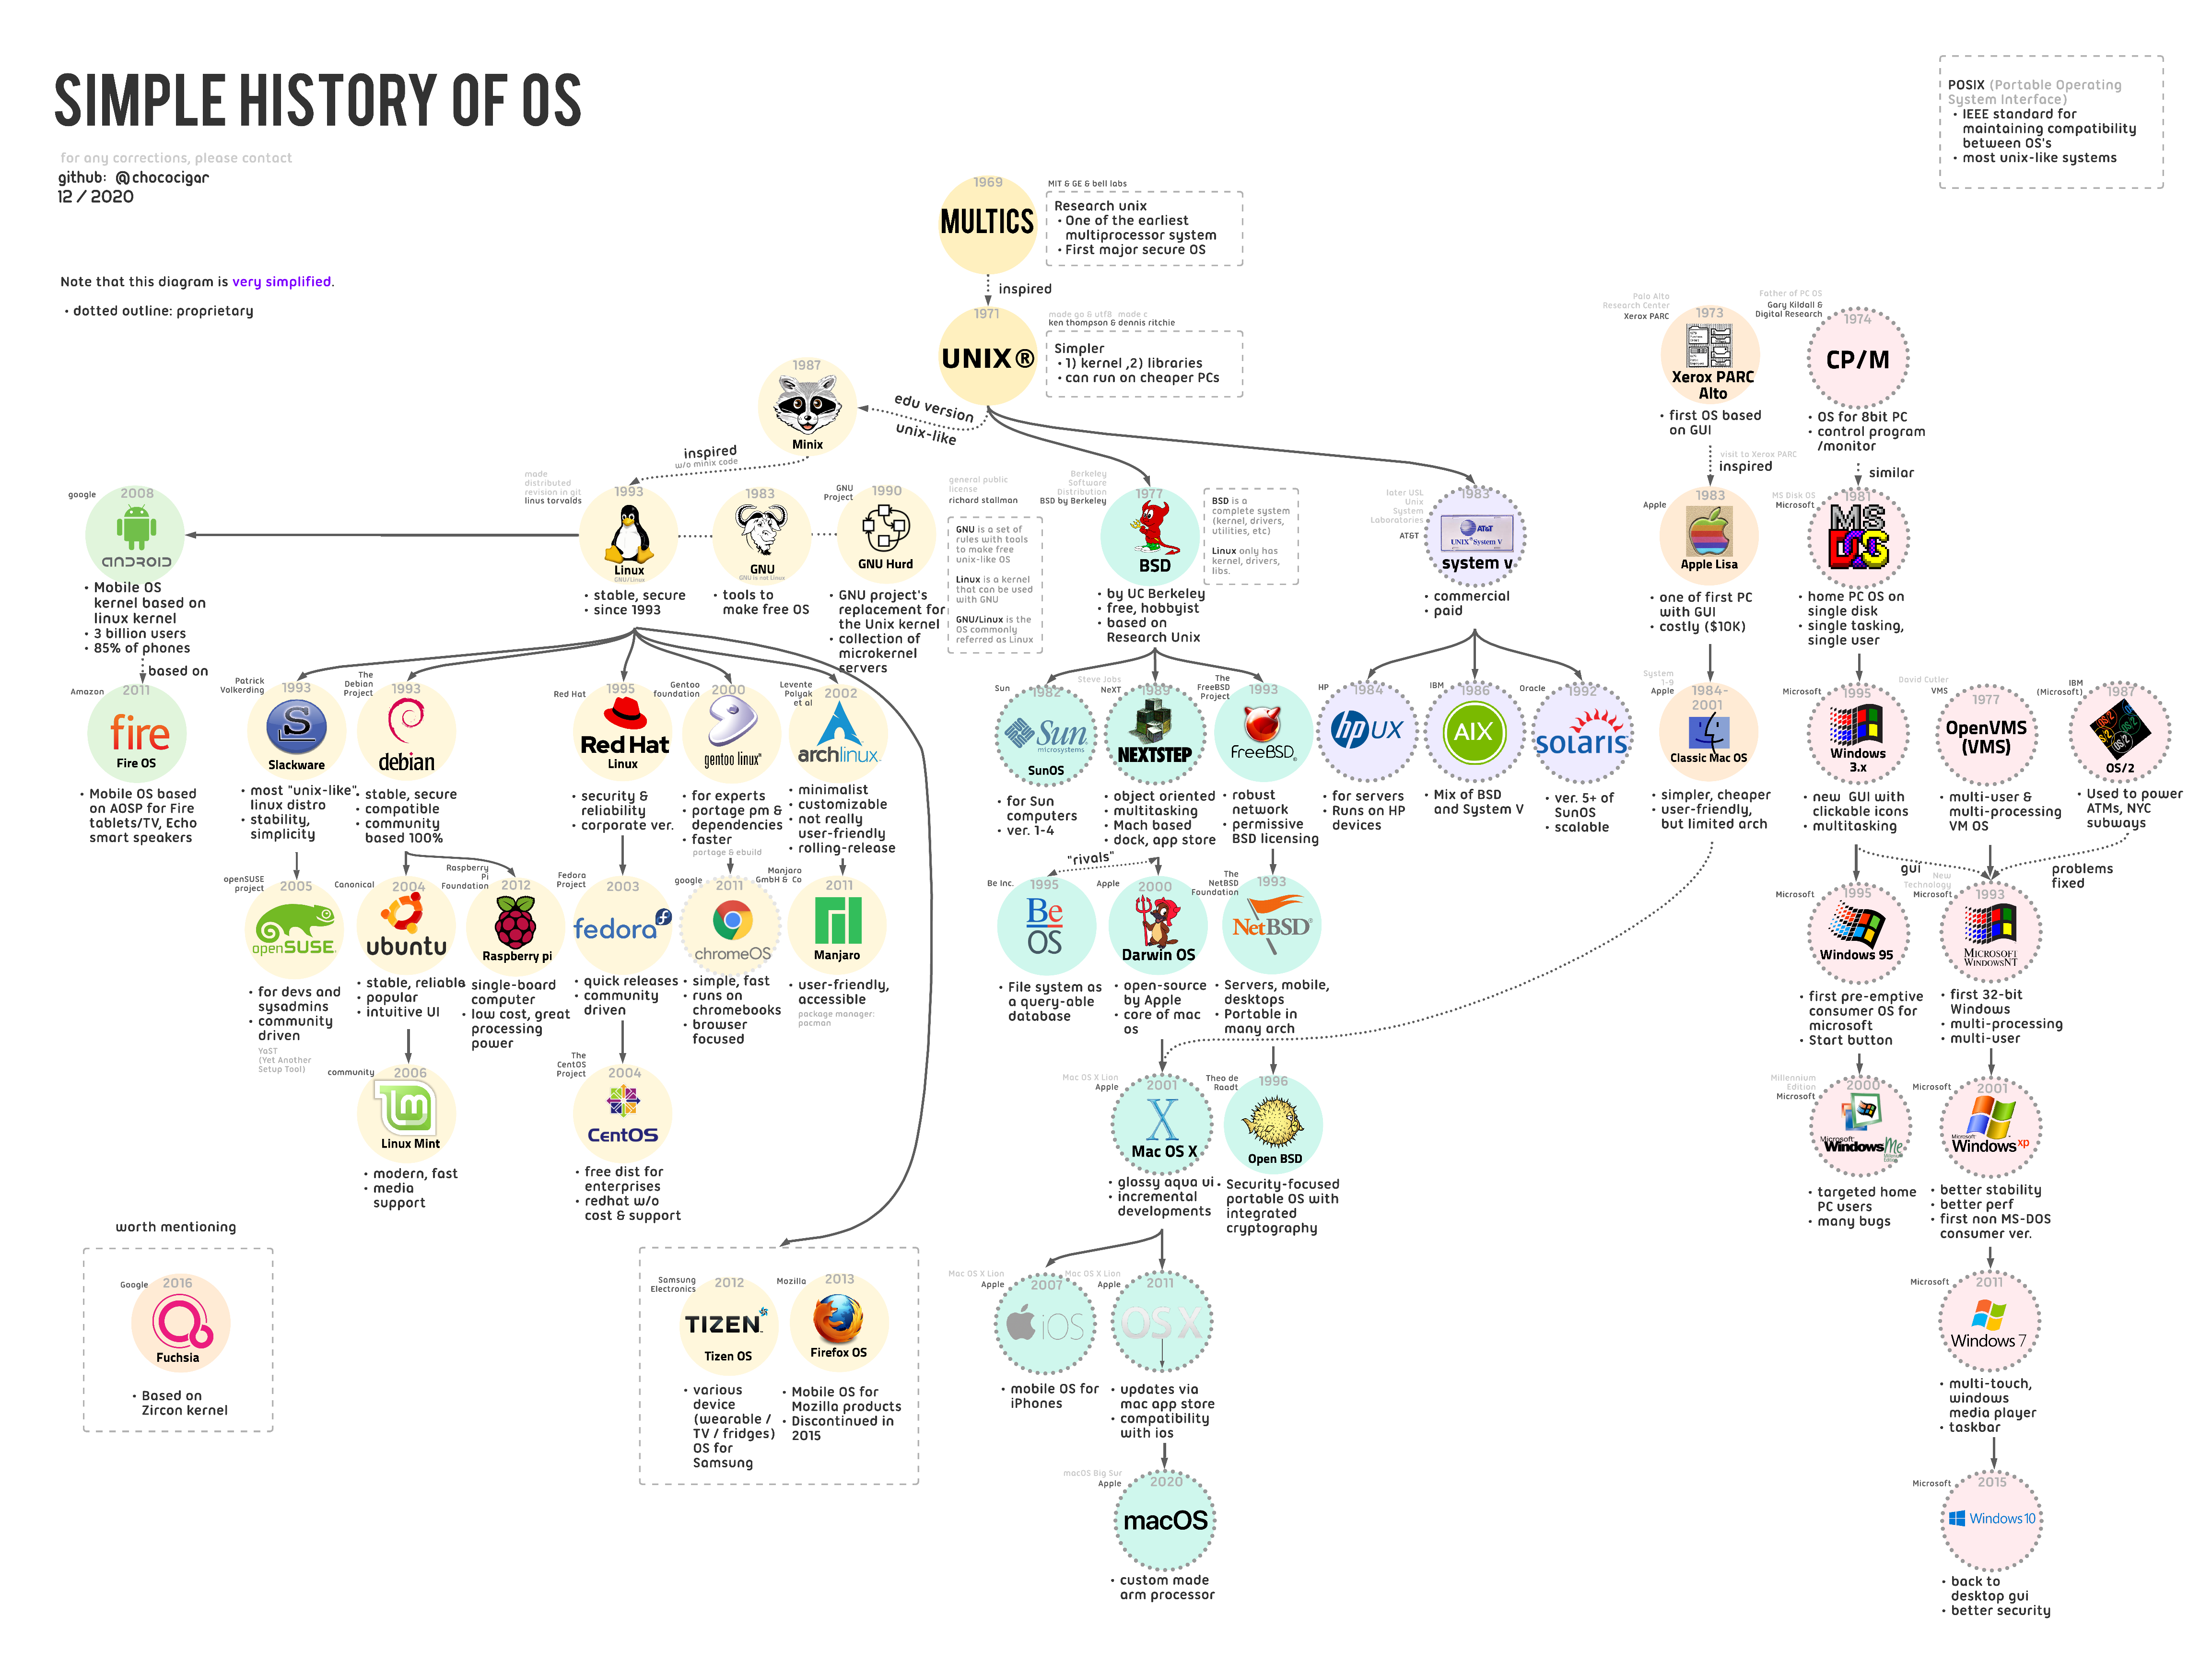
\includegraphics[width=9cm]{image/history_of_os}
    \end{frame}

    \begin{frame}
        \transdissolve
        \frametitle{Historique de Linux}
        \framesubtitle{Linux, historique des single/multi users OS}
        Multi user au sens \textit{Time-Sharing}, \textit{i.e.}, plus d'un utilisateur en même temps.

        Les premiers OS Multi user était OS/360 d'IBM dans les années 60.
        Un concurrent est développé par Bell Labs, une filiale d'AT\&T (Avant le démantèlement en 1982), c'est Unix en 1969.

        Linux est ainsi multi user dès le début.
        Par opposition à Windows, qui par défaut (sans RDP ni bricolage), ne l'est pas.
        C'est Windows® Server qui est multi user.
        \bigbreak
        Cette différence est cruciale, car elle a fait de cet OS un candidat idéal pour les serveurs (Web, BDD, \textit{etc}).
    \end{frame}

    \begin{frame}
        \footnotetext{Why Linux runs 90 percent of the public cloud workload, \url{https://www.cbtnuggets.com/blog/certifications/open-source/why-linux-runs-90-percent-of-the-public-cloud-workload}}
        \footnotetext{\label{cbt}When everything is in the cloud, does the OS matter?, \url{https://www.redhat.com/en/blog/when-everything-cloud-does-os-matter}}
        \footnotetext{20 great years of Linux and supercomputer, \url{https://www.zdnet.com/article/20-great-years-of-linux-and-supercomputers/?ref=itsfoss.com}}
        \transdissolve
        \frametitle{Historique de Linux}
        \framesubtitle{Adoption}
        \begin{columns}
            \column{0.5\textwidth}
            \begin{itemize}
                \item 2018, 90 \% des serveurs du cloud tournent sous Linux\footnotemark.
                \item 2018, 70 \% des serveurs sont déployés dans le cloud\footnotemark.
                \item 2018, 62 \% de l'embarqué\cref{cbt}.
                \item 2012, 95 \% des supercalculateurs\footnotemark.
            \end{itemize}
            \column{0.5\textwidth}
            \centering
            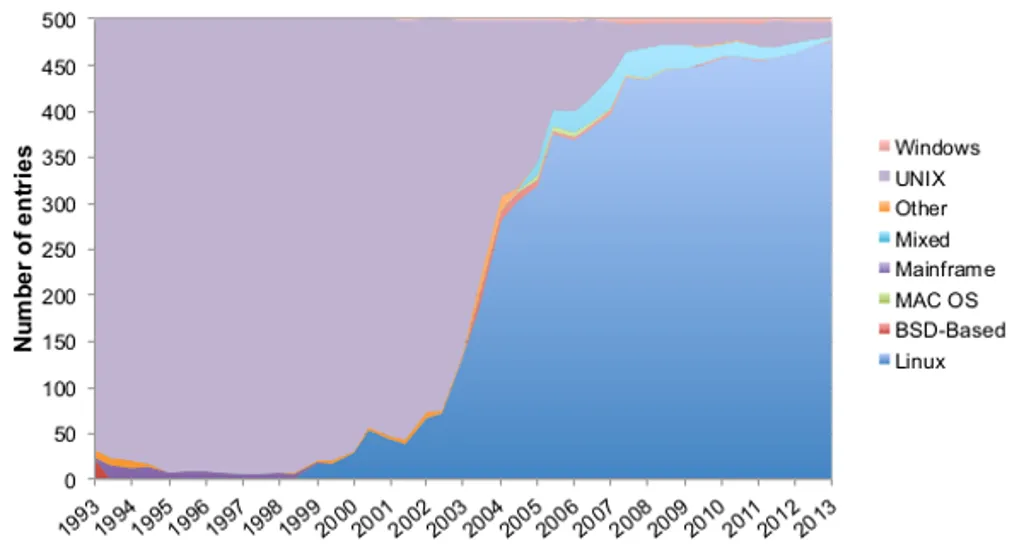
\includegraphics[width=6cm]{image/linux-supercomputer-growth}
        \end{columns}
    \end{frame}

    \subsection{Kernel et distribution}\label{subsec:kernel-et-distribution}

    \begin{frame}
        \transdissolve
        \frametitle{Les distributions}
        \framesubtitle{Définitions\footnote{Glossary, \url{https://help.ubuntu.com/community/Glossary}}}
        \begin{itemize}
            \item \textbf{Kernel} ou \textbf{Noyau}~: Le composant central d'un système d'exploitation qui contrôle tous les processus de bas niveau d'un ordinateur, tels que la gestion de la mémoire, les threads et les entrées/sorties.
            En un sens, le noyau agit comme le gardien de l'ordinateur vis-à-vis du matériel.
            Les applications font des appels système via le noyau pour demander des ressources et interagir avec le matériel.
            \item \textbf{Distribution}~: Désigne une version de GNU/Linux ou d'un autre système d'exploitation open source, bien que certaines personnes soutiennent que le terme devrait inclure les différents systèmes d'exploitation Windows® et Apple.
            Ubuntu est la version la plus populaire, mais il en existe de nombreuses autres, telles que RedHat, qui est bien connue pour les serveurs.
            La plupart des autres distros sont conçues pour un type particulier d'architecture, comme les téléphones, les netbooks, les routeurs, les serveurs, \textit{etc}.
        \end{itemize}
    \end{frame}

    \begin{frame}
        \transdissolve
        \frametitle{Les distributions}
        \framesubtitle{La timeline de toutes les distributions\footnote{FabioLolix, \url{https://github.com/FabioLolix/linuxtimeline}}\footnotestep\footnote{Put the fun back into computing. Use Linux, BSD., \url{https://distrowatch.com/}}}
        \begin{columns}
            \column{0.8\textwidth}
            Insights~:
            \begin{itemize}
                \item Les 3 plus grosses branches sont Debian, Red Hat et Ubuntu.
                \item Très nombreuses.
                \item Certaines branches meurent même après de longues années d'existence (Mandrake, Centos, \textit{etc}.).
                \item Certaines distributions passent d'une branche à l'autre.
            \end{itemize}
            Quid de l'impact sur la maintenance de la distribution~?
            \column{0.2\textwidth}
            \centering
            \includegraphics[width=1.5cm]{image/linux-all-distro-timeline}
        \end{columns}
    \end{frame}

    \begin{frame}
        \transdissolve
        \frametitle{Les distributions}
        \framesubtitle{La timeline de toutes les distributions}
        Red-Hat, filiale d'IBM, fait l'opposition entre les distributions \textit{entreprise} et les \textit{community}.
        En mettant en avant leur support de 10 ans contre 2 ans pour Fedora, une distribution communautaire de la même branche\footnote{What's the best Linux distro for you?, \url{https://www.redhat.com/en/topics/linux/whats-the-best-linux-distro-for-you}}.
        \bigbreak
        Ubuntu a un business model légèrement différent, ils proposent 5 ans de support pour les versions LTS et une extension de 10 ans dans la version payant appelée \textquote{Ubuntu Pro}\footnote{The Ubuntu lifecycle and release cadence, \url{https://ubuntu.com/about/release-cycle}}.
        \bigbreak
        Mais peut-être que l'exemple de Red-Hat n'est pas le bon, Debian, une distro communautaire également, communique un support des versions LTS de 5 ans minimum\footnote{Debian Long Term Support, \url{https://wiki.debian.org/LTS}}\ldots
    \end{frame}

    \begin{frame}
        \transdissolve
        \frametitle{Les distributions}
        \framesubtitle{La timeline des principales distributions\footnote{\label{main-distro}Philipp Leclercq, \url{https://github.com/PhilLecl/SanitizedLinuxTimeline}}}
        \centering
        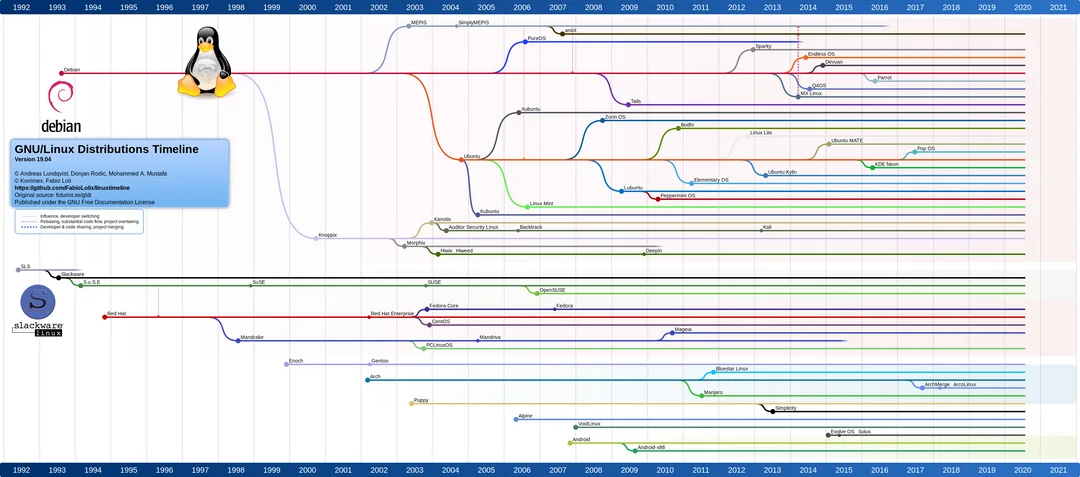
\includegraphics[width=12cm]{image/linux-main-distro-timeline}
    \end{frame}

    \begin{frame}
        \transdissolve
        \frametitle{Les distributions}
        \framesubtitle{Les licences des principales distributions\cref{main-distro}}
        \centering
        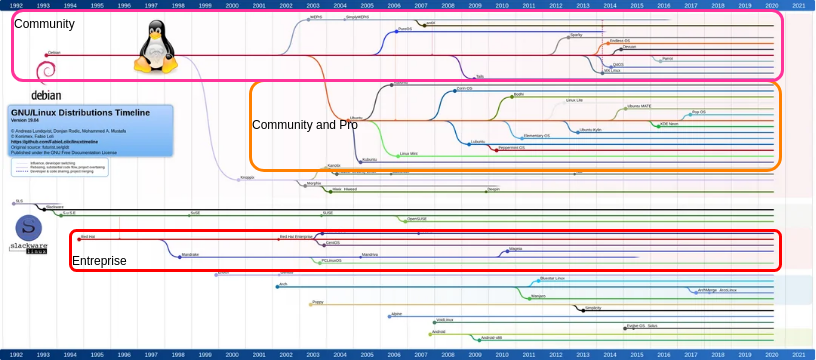
\includegraphics[width=12cm]{image/main-distro-license.drawio}
    \end{frame}

    \begin{frame}
        \transdissolve
        \frametitle{Les distributions}
        \framesubtitle{Les packages managers des principales distributions\cref{main-distro}}
        \centering
        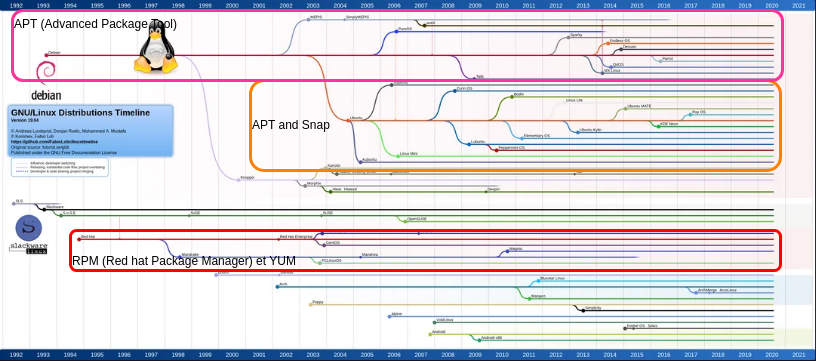
\includegraphics[width=12cm]{image/main-distro-package-manager.drawio}
    \end{frame}

    \begin{frame}
        \transdissolve
        \frametitle{Les distributions}
        \framesubtitle{Une aide pour choisir sa distribution}
        Le site Distrowatch propose un utilitaire pour trouver des distributions candidates en fonction d'un large nombre de critères, \url{https://distrowatch.com/search.php}.
        \bigbreak
        \centering
        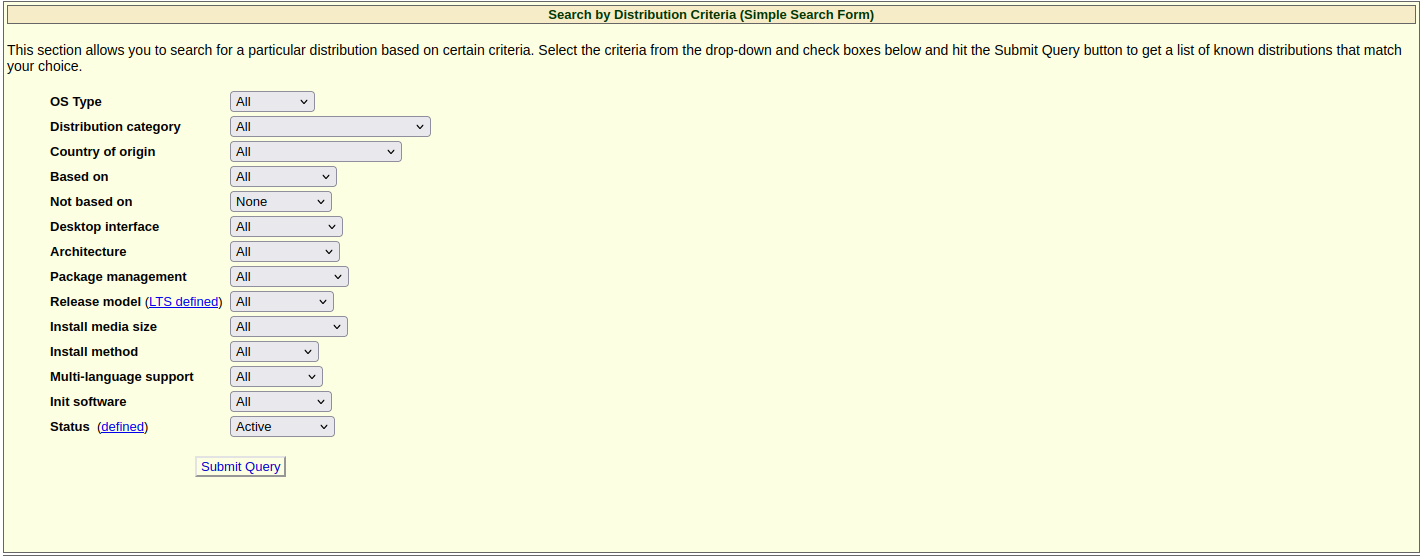
\includegraphics[width=12cm]{image/distrowatch-search}
    \end{frame}

    \begin{frame}
        \transdissolve
        \frametitle{Les distributions}
        \framesubtitle{Une aide pour choisir sa distribution}
        Admettons que tous les 2/3 packages managers mainstreams se valent.
        \bigbreak
        Un des critères différenciant, en plus du support que nous avons vu, est l'architecture.
        \bigbreak
        Qu'est-ce que le critère \textquote{architecture} et pourquoi est-ce important lors d'une migration~?
        \pause
        \bigbreak
        \begin{itemize}
            \item Une modernisation d'un hardware vieillissant qui peut être remplacé par une machine virtuelle faisant tourner les mêmes applications.
            \item Un hardware qui n'est plus supporté par la distribution actuelle et doit donc migrer.
        \end{itemize}
        Dans les 2 exemples, avoir une même architecture permettra ainsi une migration plus \textit{lean}.
        Sans rewrite, voire, sans recompilation.
    \end{frame}

    \begin{frame}
        \transdissolve
        \frametitle{Les distributions}
        \framesubtitle{Des critères manquants~?}
        Y-a-t-il des critères pertinents qui pourraient manquer~?
        \bigbreak
        \centering
        
\includegraphics[width=6cm]{image/question-mark}
    \end{frame}

    \begin{frame}
        \transdissolve
        \frametitle{Les distributions}
        \framesubtitle{Des critères manquants~?}
        L'énorme succès d'une distribution à part, Alpine Linux, pousser par les technologies de virtualisation et de conteneurisation.
        \bigbreak
        Une des premières phrases de présentation est \textit{Alpine Linux is built around musl libc and busybox. A container requires no more than 8 MB and a minimal installation to disk requires around 130 MB of storage.}\footnote{About, \url{https://alpinelinux.org/about/}}.
        \bigbreak
        De leur analyse, qui est sûrement la bonne, leur succès vient du compilateur musl et de la librairie C libc musl.
    \end{frame}

    \begin{frame}
        \transdissolve
        \frametitle{Les distributions}
        \framesubtitle{Des critères manquants~?}
        Red-Hat recrute beaucoup d'experts de LLVM ces dernières années\footnote{Red Hat Is Hiring More LLVM Compiler Engineers, \url{https://www.phoronix.com/news/Red-Hat-More-LLVM-Engineers}}.

        Certaines distributions peuvent ou sont compilé avec LLVM comme FreeBSD\footnote{Building FreeBSD with clang/llvm, \url{https://wiki.freebsd.org/BuildingFreeBSDWithClang}}, Chimera\footnote{About Chimera Linux, \url{https://chimera-linux.org/about/}}, OpenMandriva\footnote{La communauté OpenMandriva annonce la disponibilité d'OpenMandriva Lx 4.0, \url{https://linux.developpez.com/actu/266344/La-communaute-OpenMandriva-annonce-la-disponibilite-d-OpenMandriva-Lx-4-0-qui-apporte-de-nombreuses-nouveautes-liees-a-LLVM-Clang/}}\ldots
    \end{frame}

    \begin{frame}
        \transdissolve
        \frametitle{Les distributions}
        \framesubtitle{Plusieurs combinaisons de compilateurs et libraries C}
        \centering
        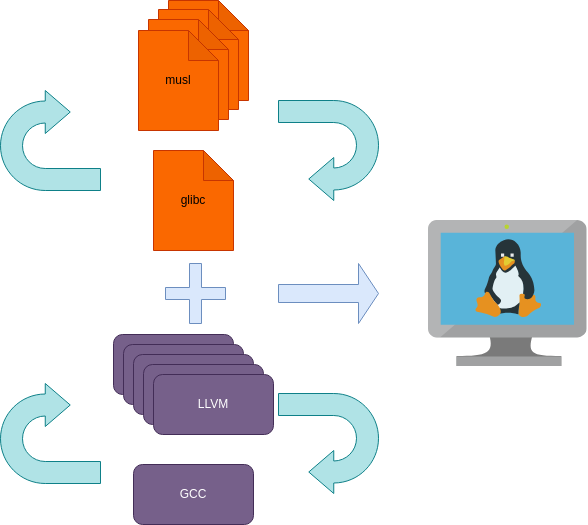
\includegraphics[width=8cm]{image/interchange-lib-compiler.drawio}
    \end{frame}

    \begin{frame}
        \transdissolve
        \frametitle{Les distributions}
        \framesubtitle{Conclusion}
        \begin{columns}
            \column{0.6\textwidth}
            Une distribution Linux est construite de manière modulaire~:
            \begin{itemize}
                \item Version de noyau.
                \item Packages manager.
                \item Architecture.
                \item Licence.
                \item Support.
                \item Librairie C~.
                \item Compilateur.
                \item \textit{Many more}.
            \end{itemize}
            \column{0.4\textwidth}
            \centering
            
\includegraphics[width=5.5cm]{image/craftsman-focused}
        \end{columns}
        \bigbreak
        À vous de trouver la meilleure combinaison pour vos besoins.
    \end{frame}


    \section{Shell et commandes de base}\label{sec:shell-and-command}

    \subsection{Shell}\label{subsec:shell}

    \begin{frame}
        \transdissolve
        \frametitle{Shell}
        \framesubtitle{Qu'est-ce~?}
        Shell c'est~:
        \begin{itemize}
            \item C'est un exécutable.
            \item Un interpréteur de ligne de commande.
            Ne pas confondre avec des Shell spécifique comme le Python Shell ou le MySQL Shell qui interagissent spécifiquement avec ces applications.
            \item Et donc un interpréteur de scripts Shell.
            \item C'est une interface entre l'OS et l'humain.
            \item Existe sur la plupart des plateformes Linux, Unix, Windows® (\lstinline{Bash}, installé avec Git par exemple), \textit{etc}.
            \item Une portabilité poussée par une standardisation, comme la standardisation POSIX~.
            \item Des Shells plus \textit{user friendly} et plus lourds comme \lstinline{zsh}.
            \item Des Shells éxotiques comme \lstinline{tcsh} et \lstinline{csh}.
        \end{itemize}
    \end{frame}

    \begin{frame}[fragile]
        \transdissolve
        \frametitle{Shell}
        \framesubtitle{Qu'est-ce~?}
        2 Shells sous une même distribution \textquote{légère} comme Alpine Linux~:
        \begin{lstlisting}[language=bash]
root@71641013d445:/usr/src/celia# sh
# ls
 Dockerfile       README.pdf         UML-Sequence.drawio       celia.ipynb
# which sh
/usr/bin/sh
# which ls
/usr/bin/ls
# bash
root@71641013d445:/usr/src/celia# which bash
/usr/bin/bash
root@71641013d445:/usr/src/celia# which ls
/usr/bin/ls
root@71641013d445:/usr/src/celia# ls
 Dockerfile       README.pdf         UML-Sequence.drawio       celia.ipynb
        \end{lstlisting}
        \bigbreak
        Comment interpréter ce code~?
    \end{frame}

    \begin{frame}
        \transdissolve
        \frametitle{Shell}
        \framesubtitle{Qu'est-ce~?}
        \begin{itemize}
            \item \lstinline{sh} et \lstinline{bash} appellent les mêmes exécutables.
            \item Shell n'est qu'une interface.
            \item Même dans une distribution \textquote{lightweight}, il y a 2 interpréteurs Shell~!
        \end{itemize}
        \bigbreak
        \lstinline{bash}, n'est pas installé par défault sur la dernière version de FreeBSD 14, uniquement \lstinline{sh}.
        Qu'en penser~?
        \bigbreak
        \centering
        
\includegraphics[width=3cm]{image/guy-in-front-of-desktop}
    \end{frame}

    \begin{frame}
        \transdissolve
        \frametitle{Shell}
        \framesubtitle{Bourne Shell VS Bourne Again Shell\footnote{Difference between sh and bash, \url{https://www.geeksforgeeks.org/difference-between-sh-and-bash/}}}
        \begin{footnotesize}
            \begin{table}[h!]
                \centering
                \begin{tabular}{|p{5.5cm}|p{5.5cm}|}
                    \hline
                    \textbf{bash}                                     & \textbf{sh}                               \\ \hline
                    Bourne Again SHell                                & SHell                                     \\ \hline
                    Developed by Brain Fox                            & Developed by Stephen R. Bourne            \\ \hline
                    Successor of sh                                   & Predecessor of bash                       \\ \hline
                    bash is the default SHELL                         & sh is not the default SHELL               \\ \hline
                    \lstinline{\#\!/bin/bash}                         & \lstinline{\#\!/bin/sh}                   \\ \hline
                    It has more functionality with up-gradation       & It has less functionality                 \\ \hline
                    Supports job controls                             & Does not support job control              \\ \hline
                    bash is not a valid POSIX shell                   & sh is a valid POSIX shell                 \\ \hline
                    Easy to use                                       & Not as easy as bash                       \\ \hline
                    Less portable than sh                             & More portable than bash                   \\ \hline
                    Extended version of language                      & Original language                         \\ \hline
                    Bash scripting is scripting specifically for Bash & Shell scripting is scripting in any shell \\ \hline
                    Supports command history                          & Does not support command history          \\ \hline
                \end{tabular}
            \end{table}
        \end{footnotesize}
    \end{frame}

    \begin{frame}
        \transdissolve
        \frametitle{Shell}
        \framesubtitle{Bourne Shell VS Bourne Again Shell}
        Peut-on lister les avantages/inconvénients de l'un et l'autre~?
        \bigbreak
        \centering
        
\includegraphics[width=6cm]{image/question-mark}
    \end{frame}

    \begin{frame}
        \transdissolve
        \frametitle{Shell}
        \framesubtitle{Le poid de cette interface\footnote{Exigences matérielles pour utiliser Ubuntu, \url{https://doc.ubuntu-fr.org/exigences_minimales}}}
        Minimum 30 Go d'espace disque disponible pour une installation avec GNOME contre 5 Go ou 6 Go pour une installation Server ou Cloud.
        \bigbreak
        L'absence de bureau, avoir uniquement cette interface, est une des raisons de cette différence de taille.

        L'interface graphique n'est donc pas installé dans les distributions dédiées aux serveurs.
        Shell et l'accès Shell distant sécurisé \lstinline{SSH} (Secure SHell), sont utilisés.
        Un client SSH comme Putty, SSH de GitBASH sous Windows® ou un terminal sous Linux permettent d'accéder à un server Linux.
        \bigbreak
        GitBash permet d'unifier les deux environnements Linux et Windows, de pratiquer le Bash sur toute plateforme.
    \end{frame}

    \begin{frame}
        \transdissolve
        \frametitle{Shell}
        \framesubtitle{Pourquoi a-t-on un Shell ou l'autre~?}
        Quand je me connecte avec mon utilisateur, j'ai souvent \lstinline{bash} comme Shell.
        Pourquoi pas \lstinline{sh}~?
        \bigbreak
        \centering
        
\includegraphics[width=6cm]{image/question-mark}
    \end{frame}

    \begin{frame}[fragile]
        \transdissolve
        \frametitle{Shell}
        \framesubtitle{Pourquoi a-t-on un Shell ou l'autre~?}
        Probablement, l'administrateur système a créé votre utilisateur en spécifiant \lstinline{bash} comme Shell.
        \bigbreak
        Si on lit l'aide de la commande \lstinline{useradd}~:
        \begin{lstlisting}[language=bash]
$ useradd -h | grep shell
  -s, --shell SHELL               interpréteur de commandes de connexion du nouveau compte
        \end{lstlisting}
        \bigbreak
        Un exemple de commande devient donc~:
        \begin{lstlisting}[language=bash]
$ useradd -s /bin/bash -m -d $/home/digiformateur digicomp
        \end{lstlisting}
        \bigbreak
        \lstinline{/bin/bash} passé à l'option \lstinline{-s} permet de spécifier le Shell.
    \end{frame}

    \begin{frame}
        \transdissolve
        \frametitle{Shell}
        \framesubtitle{Naviguer dans les commandes}
        \begin{itemize}
            \item \lstinline{history}~: Affiche l'historique des commandes.
            \item Ctrl+c~: Arrête l'exécution d'une commande.
            \item \emoji{up-arrow}~: Rappelle la dernière commande.
            \item \emoji{down-arrow}~: Rappelle la commande suivante.
            \item Ctrl+r~: Recherche dans l'historique des commandes.
            \item \lstinline{\\}~: Permet de continuer une commande sur la ligne d'après.
            \item \lstinline{\&}~: Lancer une commande en arrière-plan.
            \item Ctrl+z~: Mettre une commande en pause.
            \item \lstinline{fg}~: Reprendre une commande en pause.
            \item \lstinline{bg}~: Reprendre une commande en pause en arrière-plan.
        \end{itemize}
    \end{frame}

    \begin{frame}
        \transdissolve
        \frametitle{Shell}
        \framesubtitle{Gérer plusieurs commandes en parallèle avec \lstinline{tmux}\footnote{\label{tmux}Tmux (terminal multiplexer), \url{https://www.redhat.com/sysadmin/introduction-tmux-linux}}}
        \lstinline{tmux} est un multiplexeur de terminal, \textit{i.e.}, permet d'ouvrir plusieurs fenêtres dans un terminal.
        Chacune faisant tourner un processus.
        \begin{footnotesize}
            \begin{table}[ht]
                \centering
                \begin{tabular}{|p{3.5cm}|p{8cm}|}
                    \hline
                    \textbf{Commande}         & \textbf{Description}                                                            \\
                    \hline
                    Ctrl+b puis D             & Détacher de la session courante                                                 \\
                    \hline
                    Ctrl+b puis \%            & Diviser la fenêtre en deux volets horizontalement                               \\
                    \hline
                    Ctrl+b puis ``            & Diviser la fenêtre en deux volets verticalement                                 \\
                    \hline
                    Ctrl+b puis Flèche        & Se déplacer entre les volets                                                    \\
                    \hline
                    Ctrl+b puis X             & Fermer le volet                                                                 \\
                    \hline
                    Ctrl+b puis C             & Créer une nouvelle fenêtre                                                      \\
                    \hline
                    Ctrl+b puis N ou P        & Passer à la fenêtre suivante ou précédente                                      \\
                    \hline
                    Ctrl+b puis 0 (1,2\ldots) & Aller à une fenêtre spécifique par numéro                                       \\
                    \hline
                    Ctrl+b puis :             & Entrer dans la ligne de commande pour taper des commandes (avec autocomplétion) \\
                    \hline
                    Ctrl+b puis ?             & Voir tous les raccourcis clavier (appuyer sur Q pour quitter)                   \\
                    \hline
                    Ctrl+b puis W             & Ouvrir un panneau pour naviguer entre les fenêtres de plusieurs sessions        \\
                    \hline
                \end{tabular}
            \end{table}
        \end{footnotesize}
    \end{frame}

    \begin{frame}
        \transdissolve
        \frametitle{Shell}
        \framesubtitle{Gérer plusieurs commandes en parallèle avec \lstinline{tmux}\cref{tmux}}
        Par exemple pour monitorer les ressource avec \lstinline{top} dans le terminal de droite, pendant qu'on la commande dans celui de gauche.
        \bigbreak
        \centering
        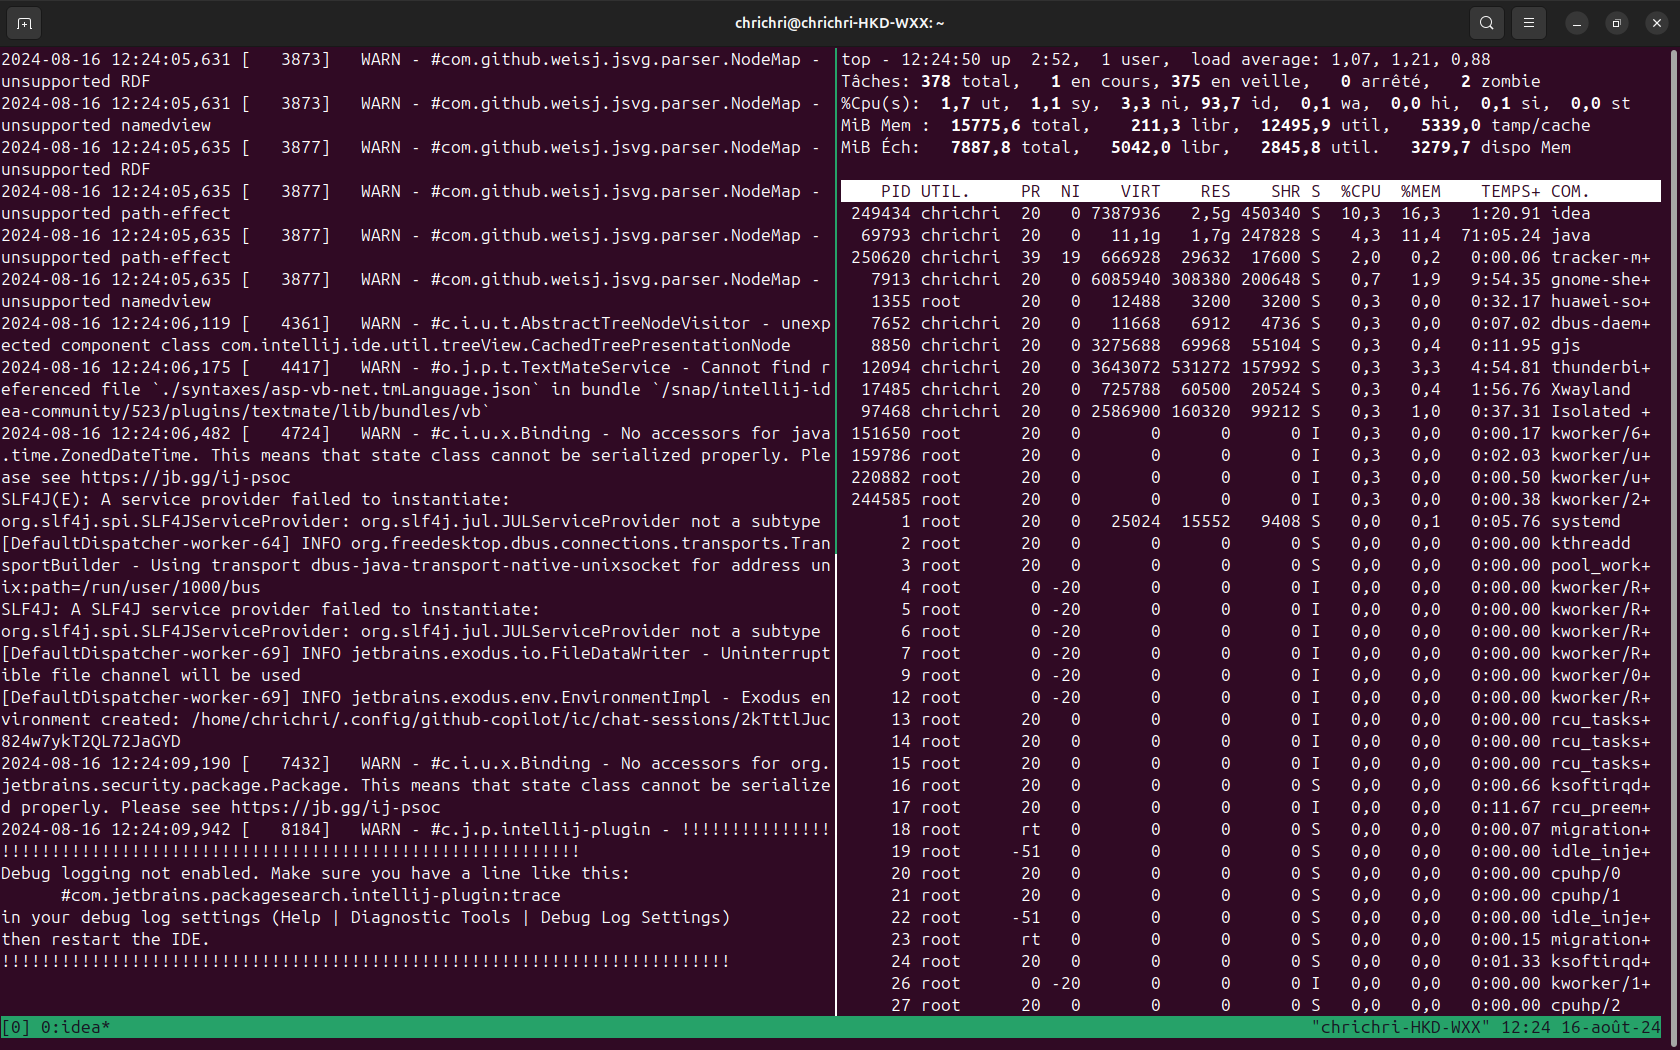
\includegraphics[width=10.3cm]{image/tmux-illustration}
    \end{frame}

    \begin{frame}[fragile]
        \transdissolve
        \frametitle{Shell}
        \framesubtitle{Gérer plusieurs commandes en parallèle avec \lstinline{nohup}}
        \lstinline{nohup} vient de NO Hang UP, c'est une commande qui permet de lancer une autre commande en arrière-plan sans qu'elle soit interrompue par la fermeture de la session Shell.
        Idéale donc pour les longs processus.
        L'output de la commande va par défault dans le fichier \lstinline{nohup.out}.
        \bigbreak
        Il suffit de préfixer la commande par \lstinline{nohup} et d'ajouter un \lstinline{&} pour libérer le terminal.
        \lstinline{nohup} indique le PID pour pouvoir stopper la commande au besoin et quand la commande est terminée, si elle s'est arrêtée (Termine <code retour>) prématurément ou normalement (Fini).
        \begin{lstlisting}[language=bash]
$ nohup ls &
[1] 279343
nohup: les entrées sont ignorées et la sortie est ajoutée à 'nohup.out'
[1]+  Fini                    nohup ls
$ tail -n 3 nohup.out
technip
Téléchargements
ts-test
        \end{lstlisting}
    \end{frame}

    \begin{frame}
        \transdissolve
        \frametitle{Shell}
        \framesubtitle{Secure SHell (SSH)}
        La machine Linux à administrer sera le plus souvent dans un cloud, une salle serveur, un data center, elle sera distante.
        Dans une infrastructure sécurisée.
        \bigbreak
        Mais avec un user, un Shell par défaut, et un protocole sécurisé comme le SSH~.
        Nous allons pouvoir nous connecter et l'administrer.
        \bigbreak
        Les bonnes pratiques sont d'utiliser les clés SSH uniquement, pas de connexion SSH avec l'utilisateur root,
        Tutoriel utile~:
        \begin{itemize}
            \item \href{https://phoenixnap.com/kb/generate-setup-ssh-key-ubuntu}{Configuration du login SSH sur Ubuntu}
        \end{itemize}
        \bigbreak
        \centering
        
\includegraphics[width=3cm]{image/guy-in-front-of-desktop}
    \end{frame}

    \begin{frame}
        \frametitle{Shell}
        \framesubtitle{Sécurisation du SSH avec la cryptographie asymétrique}
        \transdissolve
        Pourquoi est-ce plus sécure d'utiliser une clé SSH plutôt qu'un mot de passe~?
        \bigbreak
        Quels algorithmes et taille de clés sont recommandés~?
        \pause
        \bigbreak
        Sur le site \url{https://jadaptive.com/ssh-key-management/the-benefits-of-ssh-key-authentication/} on trouve~:
        \begin{columns}
            \begin{column}{0.6\textwidth}
                \begin{itemize}
                    \item Le mot de passe doit être communiqué à chaque connexion, il est donc plus vulnérable à une interception/sniffing/MITHM~.
                    La clé privée reste sur le client, elle n'est pas communiquée.
                    \item La clé SSH est plus complexe à deviner qu'un mot de passe.
                    \item On peut automatiser des taches depuis la machine cliente avec la clé SSH~.
                \end{itemize}
            \end{column}
            \begin{column}{0.4\textwidth}
                \centering
                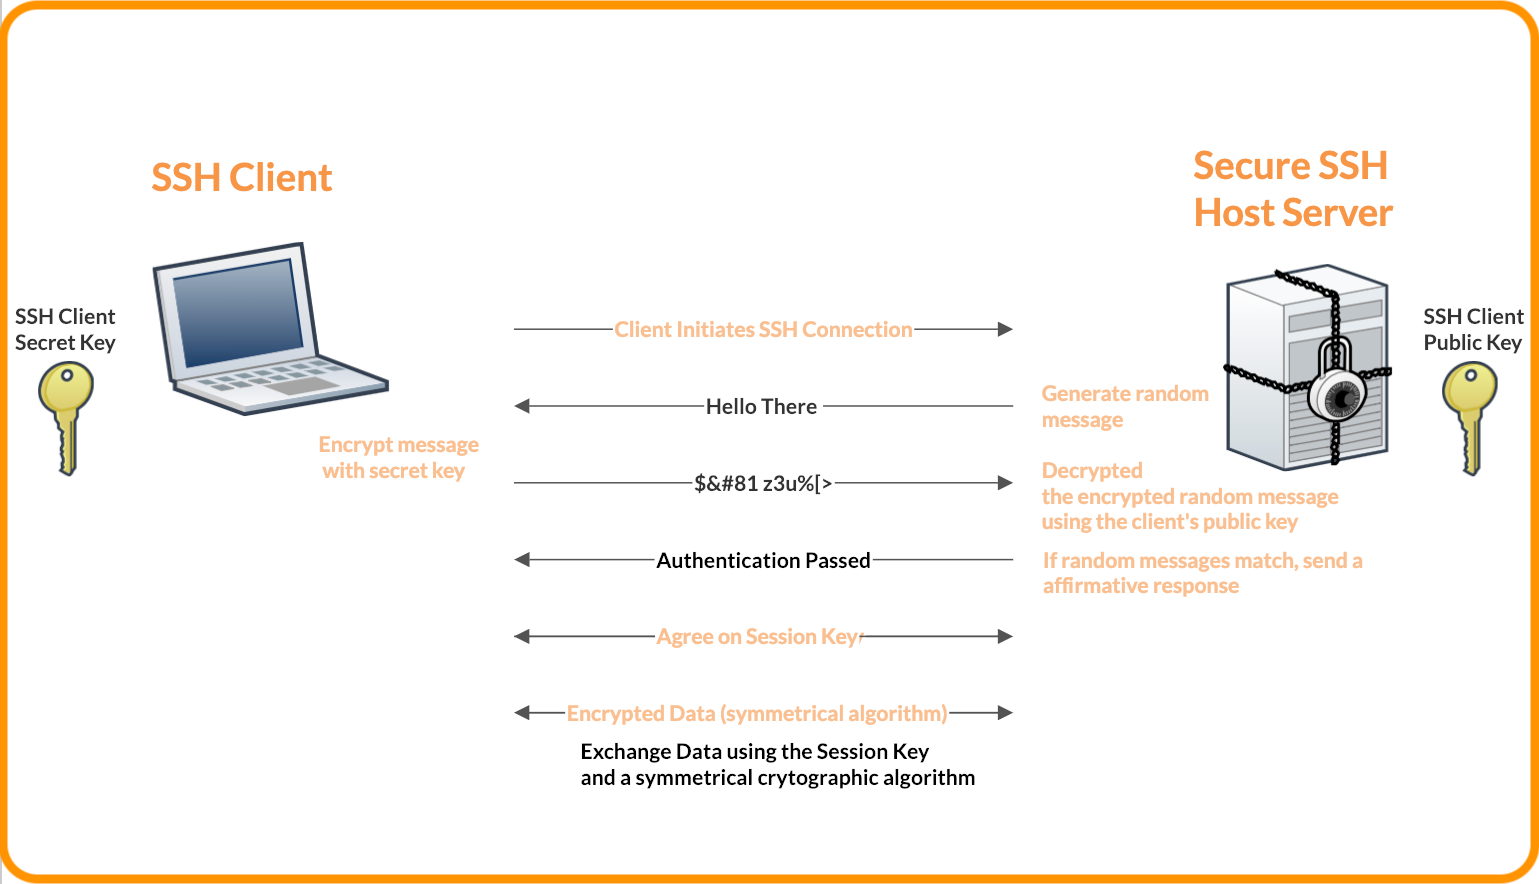
\includegraphics[width=5cm]{image/ssh-key-diagram} \\ Foxpass\footnotemark \\
            \end{column}
        \end{columns}
    \end{frame}

    \begin{frame}
        \frametitle{Shell}
        \framesubtitle{Sécurisation du SSH avec la cryptographie asymétrique}
        \transdissolve
        Exercice \execcounterdispinc{}~:
        Restreindre l'accès à la VM au SSH avec une clé SSH, aucun mot de passe.
        \bigbreak
        Exercice \execcounterdispinc{}~:
        Créer un user pour un de vos camarades.
        Lui donner un Shell \lstinline{sh} par défaut.
        Configurer lui communiquer les clés SSH pour qu'il puisse se connecter.
    \end{frame}

    \begin{frame}[fragile]
        \transdissolve
        \frametitle{Shell}
        \framesubtitle{Une des solutions (commande à exécuter sur la VM)}
        Commande pour configurer la VM~:
        \begin{lstlisting}[language=bash][fragile]
# Configure SSH
sudo sed -i 's/PermitRootLogin yes/PermitRootLogin no/' /etc/ssh/sshd_config
sudo sed -i 's/PasswordAuthentication yes/PasswordAuthentication no/' /etc/ssh/sshd_config
# Restart SSH with the new configuration
sudo systemctl restart sshd
# Create the .ssh directory and the authorized_keys file
mkdir -p ~/.ssh
touch ~/.ssh/authorized_keys
# Add the public key to the authorized_keys file
echo "ssh-rsa AAAAB3NzaC1yc2EAAAADAQABAAABgQDQ8z4... chrichri@localhost" >> ~/.ssh/authorized_keys
        \end{lstlisting}
        \begin{center}
            
\includegraphics[width=2cm]{image/digicomp-lightbulb} \\ Expliquer chaque commande \\
        \end{center}
    \end{frame}

    \begin{frame}[fragile]
        \frametitle{Shell}
        \framesubtitle{Exemple de sécurisation des clés et des secrets sous Linux}
        \transdissolve
        Par défaut, Ubuntu desktop s’installe sur une partition non
        chiffrée (encrypter, ce n’est pas français on dit chiffrer~!~).
        Tout document peut donc être lu avec un disque de
        démarrage (live CD, USB bootable, etc) ou si le disque dur
        est extrait et lu (vol, perte du desktop\ldots).
        \bigbreak
        Avec le package \lstinline{ecryptfs-utils} on peut chiffrer une partition~:
        \begin{lstlisting}[language=bash]
$ sudo apt-get install ecryptfs-utils
$ ecryptfs-setup-private
$ cp -r .ssh/ Private/ # Pour proteger les clés SSH on les déplace
$ ln -s /home/<mon user Ubuntu>/Private/.ssh/ . # Lien symbolique
        \end{lstlisting}
        Output~:
        \begin{lstlisting}
$ ls ~/.ssh -d -lha
lrwxrwxrwx 1 chrichri chrichri 28 janv. 14 21:27 /home/chrichri/.ssh -> /home/chrichri/Private/.ssh/
        \end{lstlisting}
        Il utilise le mot de passe de la session pour chiffrer/déchiffrer.
        Si la session n'est pas ouverte, les données sont chiffrées.
    \end{frame}

    \subsection{Commandes de base}\label{subsec:commandes-de-base}

    \begin{frame}
        \transdissolve
        \frametitle{Commandes de base}
        \framesubtitle{Commandes de base}
        \begin{itemize}
            \item \lstinline{ls}~: Liste les fichiers et répertoires.
            \item \lstinline{cd}~: Change de répertoire.
            \item \lstinline{pwd}~: Affiche le répertoire courant.
            \item \lstinline{cp}~: Copie des fichiers et des répertoires.
            \item \lstinline{mv}~: Déplace des fichiers et des répertoires.
            \item \lstinline{rm}~: Supprime des fichiers et des répertoires.
            \item \lstinline{mkdir}~: Crée des répertoires.
            \item \lstinline{cat}~: Affiche le contenu d'un fichier.
            \item \lstinline{head}~: Affiche les premières lignes d'un fichier.
            \item \lstinline{tail}~: Affiche les dernières lignes d'un fichier.
            \item \lstinline{touch}~: Crée un fichier vide.
            \item \lstinline{echo}~: Affiche une chaîne de caractères.
            \item \lstinline{du}~: Affiche l'espace disque utilisé par les fichiers.
        \end{itemize}
    \end{frame}

    \begin{frame}[fragile]
        \transdissolve
        \frametitle{Commandes de base}
        \framesubtitle{Les options}
        Mais souvent, une commande seule ne suffit pas, il faut utiliser des options.

        Il existe deux solutions pour découvrir ces options~:
        \begin{itemize}
            \item Utiliser l'aide de la commande.
            Le plus souvent avec l'option \lstinline{-h}, équivalente à \lstinline{--help}.
            \begin{lstlisting}[language=bash]
$ ls --help # -h c'est human readable avec ls...
            \end{lstlisting}
            \item Ce qui revient à lire la documentation de la commande avec la commande~:
            \begin{lstlisting}[language=bash]
$ man ls # Same as above
            \end{lstlisting}
        \end{itemize}
    \end{frame}

    \begin{frame}[fragile]
        \transdissolve
        \frametitle{Commandes de base}
        \framesubtitle{Busy box}
        BusyBox est un logiciel libre qui fournit une implémentation unique d'environ 200 commandes UNIX standard dans un seul fichier pour diminuer la taille de ces derniers.
        Des distributions comme Alpine Linux l'utilisent pour réduire la taille de l'OS~.
        \begin{lstlisting}[language=bash,basicstyle=\tiny\ttfamily]
$ busybox
BusyBox v1.36.1 (Ubuntu 1:1.36.1-6ubuntu3) multi-call binary.
BusyBox is copyrighted by many authors between 1998-2015.
Licensed under GPLv2. See source distribution for detailed
copyright notices.

Usage: busybox [function [arguments]...]
   or: busybox --list[-full]
   or: busybox --install [-s] [DIR]
   or: function [arguments]...

        BusyBox is a multi-call binary that combines many common Unix
        utilities into a single executable.  The shell in this build
        is configured to run built-in utilities without $PATH search.
        You don't need to install a link to busybox for each utility.
        To run external program, use full path (/sbin/ip instead of ip).

Currently defined functions:
        [, [[, acpid, adjtimex, ar, arch, arp, arping, ascii, ash, awk, base64, basename, bc, blkdiscard, blockdev, brctl, bunzip2, busybox, bzcat, bzip2, cal, cat, chgrp, chmod, chown, chpasswd, chroot, chvt, clear, cmp, cp,
        cpio, crc32, crond, crontab, cttyhack, cut, date, dc, dd, deallocvt, depmod, devmem, df, diff, dirname, dmesg, dnsdomainname, dos2unix, dpkg, dpkg-deb, du, dumpkmap, dumpleases, echo, ed,
        \end{lstlisting}
    \end{frame}
    \begin{frame}[fragile]
        \transdissolve
        \frametitle{Commandes de base}
        \framesubtitle{Busy box}
        \begin{lstlisting}[language=bash,basicstyle=\tiny\ttfamily]
        egrep, env, expand, expr, factor,
        fallocate, false, fatattr, fdisk, fgrep, find, findfs, fold, free, freeramdisk, fsfreeze, fstrim, ftpget, ftpput, getopt, getty, grep, groups, gunzip, gzip, halt, head, hexdump, hostid, hostname, httpd, hwclock, i2cdetect,
        i2cdump, i2cget, i2cset, i2ctransfer, id, ifconfig, ifdown, ifup, init, insmod, ionice, ip, ipcalc, kill, killall, klogd, last, less, link, linux32, linux64, linuxrc, ln, loadfont, loadkmap, logger, login, logname,
        logread, losetup, ls, lsmod, lsscsi, lzcat, lzma, lzop, md5sum, mdev, microcom, mim, mkdir, mkdosfs, mke2fs, mkfifo, mknod, mkpasswd, mkswap, mktemp, modinfo, modprobe, more, mount, mt, mv, nameif, nbd-client, nc, netstat,
        nl, nologin, nproc, nsenter, nslookup, nuke, od, openvt, partprobe, passwd, paste, patch, pidof, ping, ping6, pivot_root, poweroff, printf, ps, pwd, rdate, readlink, realpath, reboot, renice, reset, resume, rev, rm, rmdir,
        rmmod, route, rpm, rpm2cpio, run-init, run-parts, sed, seq, setkeycodes, setpriv, setsid, sh, sha1sum, sha256sum, sha3sum, sha512sum, shred, shuf, sleep, sort, ssl_client, start-stop-daemon, stat, static-sh, strings, stty,
        su, sulogin, svc, svok, swapoff, swapon, switch_root, sync, sysctl, syslogd, tac, tail, tar, taskset, tc, tee, telnet, telnetd, test, tftp, time, timeout, top, touch, tr, traceroute, traceroute6, true, truncate, ts, tty,
        tunctl, ubirename, udhcpc, udhcpc6, udhcpd, uevent, umount, uname, uncompress, unexpand, uniq, unix2dos, unlink, unlzma, unshare, unxz, unzip, uptime, usleep, uudecode, uuencode, vconfig, vi, w, watch, watchdog, wc, wget,
        which, who, whoami, xargs, xxd, xz, xzcat, yes, zcat
$ busybox ls
LICENSE            checkmytex.sh      compress-image.sh  dept.csv           employee.csv       sqlite-hr.sh       venv
        \end{lstlisting}
        Et s'utilise en remplaçant la commande par \lstinline{busybox <commande>}.
        \begin{lstlisting}[language=bash,basicstyle=\tiny\ttfamily]
$ busybox sha256sum employee.csv
c148c36111463e962f490742af787c1f8e49776f09d89e19f71c6cdcf220240d  employee.csv
        \end{lstlisting}
    \end{frame}

    \begin{frame}
        \transdissolve
        \frametitle{Commandes de base}
        \framesubtitle{Exercice \execcounterdispinc{}~:}
        Le but est de préparer la configuration d'un nouveau service après avoir sauvegardé l'original.
        \begin{itemize}
            \item Créer un répertoire de backup des services dans votre \textquote{home} nommé \lstinline{service-backup}.
            \item Se déplacer dans le répertoire des services \lstinline{/etc/systemd/system}.
            \item Copier un service dans \lstinline{service-backup}.
            \item Afficher le contenu du fichier copié pour vérifier ce dernier.
            \item Créer un répertoire de développement des services dans votre \textquote{home} nommé \lstinline{service-dev}.
            \item Copier le contenu de \lstinline{service-backup} dans \lstinline{service-dev}.
            \item Modifier la description du service de \lstinline{service-dev} avec un éditeur et sauvegarder.
        \end{itemize}
    \end{frame}

    \begin{frame}
        \transdissolve
        \frametitle{Commandes de base}
        \framesubtitle{Opérateurs de redirection et piping\footnote{Five ways to use redirect operators in Bash, \url{https://www.redhat.com/sysadmin/redirect-operators-bash}}}
        \begin{itemize}
            \item \lstinline{>}~: Redirige la sortie standard vers un fichier.
            \item \lstinline{>>}~: Redirige la sortie standard vers un fichier en ajoutant le contenu à la fin.
            \item \lstinline{<}~: Redirige un fichier vers l'entrée standard.
            \item \lstinline{2>}~: Redirige la sortie d'erreur vers un fichier.
            \item \lstinline{|}~: Piping, redirige la sortie standard d'une commande vers l'entrée standard d'une autre.
        \end{itemize}
        À quoi ces opérateurs peuvent-ils servir~?
        \begin{center}
            
\includegraphics[width=3cm]{image/question-mark}
        \end{center}
    \end{frame}

    \begin{frame}
        \transdissolve
        \frametitle{Commandes de base}
        \framesubtitle{Exercice \execcounterdispinc{}~:}
        Le but est de créer un fichier source d'un script Shell en y ajoutant ligne par ligne les commandes.
        \begin{itemize}
            \item Initier la création d'un script Shell nommé \lstinline{discover.sh} dans votre \textquote{home} avec un commentaire descriptif.
            \item Ajouter l'output d'un message indiquant que le current working directory va s'afficher.
            \item Ajouter la commande pour afficher le répertoire courant.
            \item Ajouter l'output d'un message indiquant que les fichiers et répertoires du répertoire courant vont s'afficher.
            \item Ajouter une commande pour lister les fichiers et répertoires du répertoire courant.
        \end{itemize}

        Inutile donc indispensable~:
        \begin{itemize}
            \item Changer de répertoire pour aller dans le répertoire courant avec le pipe.
        \end{itemize}
    \end{frame}

    \subsection{Commandes de traitement de données}\label{subsec:commandes-donnees}

    \begin{frame}
        \transdissolve
        \frametitle{Commandes de traitement de données}
        \framesubtitle{Les grands classiques}
        \begin{itemize}
            \item \lstinline{grep}~: Recherche de chaînes de caractères dans un fichier à l'aide d'une RegExp, une \textquote{Regular Expression}.
            Le nom vient de \textit{Global Regular Expression Print}.
            \item \lstinline{sed}~: Stream EDitor, éditeur de flux, permet de modifier le contenu d'un fichier.
            Le plus souvent à l'aide d'une RegExp également.
            Il peut substituer un pattern, supprimer une ligne, ajouter une ligne, \textit{etc}.
            \item \lstinline{awk}~: Traitement de texte, permet de lire un fichier ligne par ligne et de le traiter.
            Il est plus complexe, il a son propre langage de programmation.
            \item \lstinline{cut}~: Permet de découper un fichier en colonnes et de les sélectionner.
            \item \lstinline{sort}~: Trie les lignes d'un fichier.
            \item \lstinline{join}~: Joint les lignes de deux fichiers sur un champ commun.
        \end{itemize}
    \end{frame}

    \subsubsection{Piping}\label{subsubsec:piping}
    \begin{frame}
        \transdissolve
        \frametitle{Commandes de traitement de données}
        \framesubtitle{L'histoire du piping}
        Les opérateurs de redirection et le piping margent toujours évidement avec ces commandes.
        \bigbreak
        \begin{columns}
            \centering
            \column{0.2\textwidth}
            
\includegraphics[width=3cm]{image/digicomp-video}
            \column{0.8\textwidth}
            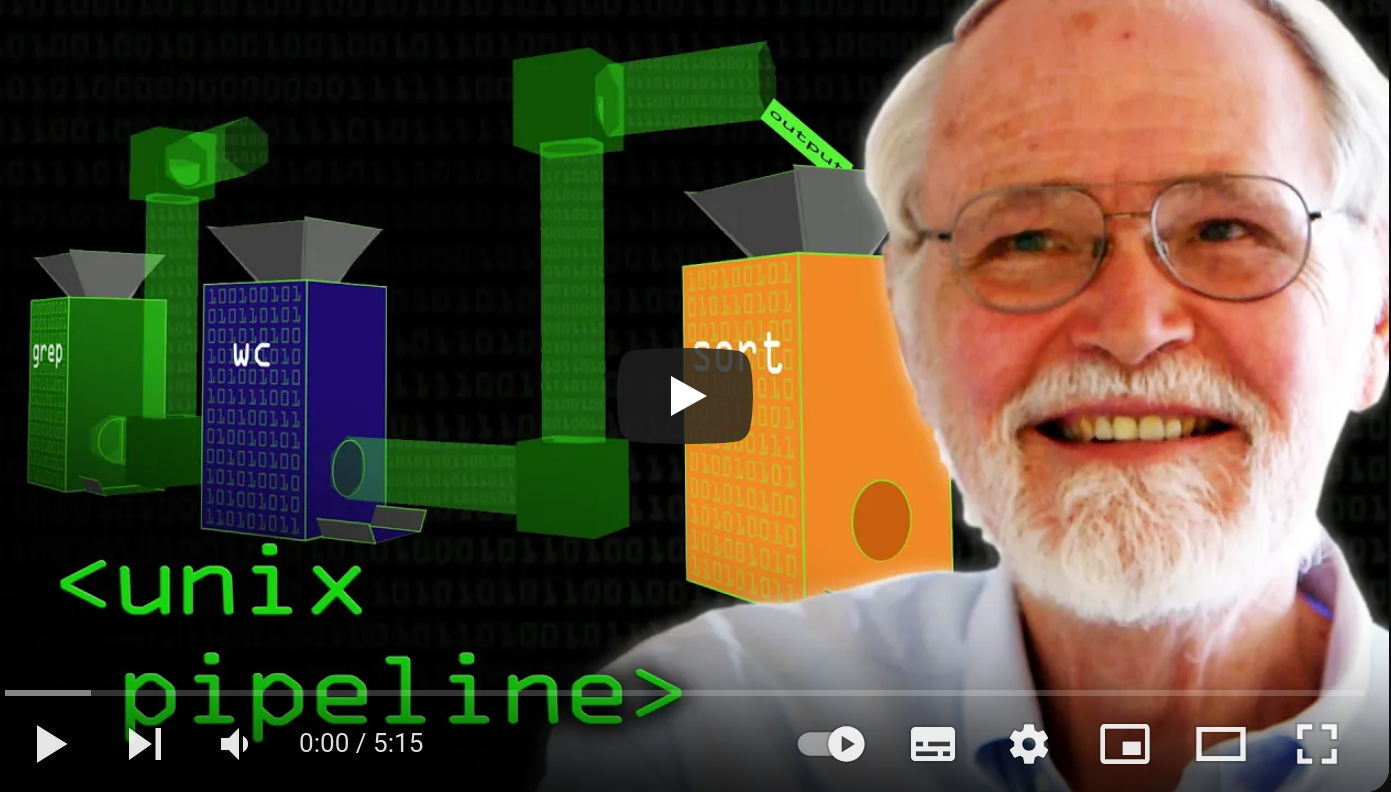
\includegraphics[width=9cm]{image/kernighan-piping-video} \\ \url{https://www.youtube.com/watch?v=bKzonnwoR2I} \\
        \end{columns}
    \end{frame}

    \subsubsection{grep}\label{subsubsec:grep}
    \begin{frame}[fragile]
        \transdissolve
        \frametitle{Commandes de traitement de données}
        \framesubtitle{\lstinline{grep}}
        Exemple chercher une adresse mail dans un fichier.
        \bigbreak
        On valide d'abord la RegExp en ligne avec un utilitaire comme \url{https://regex101.com/}.
        \bigbreak
        Par exemple, pour chercher les connexions depuis une IP dans le fichier de ProFTP (un serveur FTP)~:
        \begin{lstlisting}[language=bash,basicstyle=\tiny\ttfamily]
$ grep -P 'from\s([0-9]{1,3}.[0-9]{1,3}.[0-9]{1,3}.[0-9]{1,3})' proftpd.log.1
2023-03-05 11:35:16,736 vps19562 proftpd[663168] vps19562.dreamhostps.com (104.156.155.30[104.156.155.30]): USER anonymous: no such user found from 104.156.155.30 [104.156.155.30] to ::ffff:66.33.201.239:21
2023-03-05 13:44:22,711 vps19562 proftpd[664214] vps19562.dreamhostps.com (183.127.77.34.bc.googleusercontent.com[34.77.127.183]): USER anonymous: no such user found from 183.127.77.34.bc.googleusercontent.com [34.77.127.183] to ::ffff:66.33.201.239:21
2023-03-05 21:18:51,926 vps19562 proftpd[669957] vps19562.dreamhostps.com (182.176.228.148[182.176.228.148]): USER local: no such user found from 182.176.228.148 [182.176.228.148] to ::ffff:66.33.201.239:21
2023-03-05 21:59:46,174 vps19562 proftpd[670340] vps19562.dreamhostps.com (107.150.102.211[107.150.102.211]): USER anonymous: no such user found from 107.150.102.211 [107.150.102.211] to ::ffff:66.33.201.239:21
2023-03-06 13:36:11,788 vps19562 proftpd[681605] vps19562.dreamhostps.com (116.62.233.35.bc.googleusercontent.com[35.233.62.116]): USER anonymous: no such user found from 116.62.233.35.bc.googleusercontent.com [35.233.62.116] to ::ffff:66.33.201.239:21
2023-03-07 10:19:49,666 vps19562 proftpd[695638] vps19562.dreamhostps.com (116.62.233.35.bc.googleusercontent.com[35.233.62.116]): USER anonymous: no such user found from 116.62.233.35.bc.googleusercontent.com [35.233.62.116] to ::ffff:66.33.201.239:21
        \end{lstlisting}
    \end{frame}

    \begin{frame}[fragile]
        \transdissolve
        \frametitle{Commandes de traitement de données}
        \framesubtitle{\lstinline{grep} pour le \textquote{Pattern Matching}}
        Sinon en rajouter l'option \lstinline{-o} pour avoir uniquement le pattern qui match~:
        \begin{lstlisting}[language=bash]
$ grep -oP 'from\s(\d{1,3}.\d{1,3}.\d{1,3}.\d{1,3})' proftpd.log.1
from 104.156.155.30
from 183.127.77.34
from 182.176.228.148
from 107.150.102.211
from 116.62.233.35
from 116.62.233.35
        \end{lstlisting}
        Uniquement sur les 10 premières lignes grâce à \lstinline{head}~:
        \begin{lstlisting}[language=bash]
$ grep -oP 'from\s(\d{1,3}.\d{1,3}.\d{1,3}.\d{1,3})' <(head -n 10 proftpd.log.1)
from 104.156.155.30
from 183.127.77.34
from 182.176.228.148
from 107.150.102.211
        \end{lstlisting}
        Expliquer cette dernière commande.
    \end{frame}

    \subsubsection{sed}\label{subsubsec:sed}
    \begin{frame}[fragile]
        \transdissolve
        \frametitle{Commandes de traitement de données}
        \framesubtitle{\lstinline{sed} la substitution}
        \lstinline{sed} a son propre langage de programmation avec \lstinline{s/}\footnote{\label{sed}Sed - An Introduction and Tutorial by Bruce Barnett, \url{https://www.grymoire.com/Unix/Sed.html}}.
        \bigbreak
        On peut anonymiser le fichier en remplaçant une chaine de caractère par une autre.
        \begin{lstlisting}[language=bash,basicstyle=\tiny\ttfamily]
$ head -n 3 proftpd.log.1
2023-03-05 00:17:11,880 vps19562 proftpX[653589] vps19562.dreamhostps.com: ProFTPD 1.3.6c (maint) (built Thu Feb 27 2020 19:34:56 UTC) standalone mode STARTUP
2023-03-05 00:47:51,132 vps19562 proftpX[653845] vps19562.dreamhostps.com (aurora.probe.onyphe.net[142.4.218.114]): USER anonymous: no such user found from aurora.probe.onyphe.net [142.4.218.114] to ::ffff:66.33.201.239:21
2023-03-05 00:55:14,666 vps19562 proftpX[655268] vps19562.dreamhostps.com (hodson.probe.onyphe.net[178.32.197.87]): USER anonymous: no such user found from hodson.probe.onyphe.net [178.32.197.87] to ::ffff:66.33.201.239:21
$ head -n 3 proftpd.log.1 | sed s/vps19562.dreamhostps.com/XXX/
2023-03-05 00:17:11,880 vps19562 proftpX[653589] XXX: ProFTPD 1.3.6c (maint) (built Thu Feb 27 2020 19:34:56 UTC) standalone mode STARTUP
2023-03-05 00:47:51,132 vps19562 proftpX[653845] XXX (aurora.probe.onyphe.net[142.4.218.114]): USER anonymous: no such user found from aurora.probe.onyphe.net [142.4.218.114] to ::ffff:66.33.201.239:21
2023-03-05 00:55:14,666 vps19562 proftpX[655268] XXX (hodson.probe.onyphe.net[178.32.197.87]): USER anonymous: no such user found from hodson.probe.onyphe.net [178.32.197.87] to ::ffff:66.33.201.239:21
        \end{lstlisting}
    \end{frame}

    \begin{frame}[fragile]
        \transdissolve
        \frametitle{Commandes de traitement de données}
        \framesubtitle{\lstinline{sed} la substitution avec \lstinline{s/}\cref{sed}}
        On peut anonymiser le fichier en remplaçant une chaine de caractère par une autre.
        On peut utiliser \lstinline{sed} pour substituer un pattern, donc une RegExp, avec l'option \lstinline{-E}, par une chaîne de caractère et donc anonymiser le fichier en remplaçant les IPv4 par \textquote{xxx.xxx.xxx.xxx}~:
        \begin{lstlisting}[language=bash,basicstyle=\tiny\ttfamily]
$ head -n 3 proftpd.log.1 | sed -E 's/\[[0-9]{1,3}.[0-9]{1,3}.[0-9]{1,3}.[0-9]{1,3}\]/[xxx.xxx.xxx.xxx]/g'
2023-03-05 00:17:11,880 vps19562 proftpX[653589] vps19562.dreamhostps.com: ProFTPD 1.3.6c (maint) (built Thu Feb 27 2020 19:34:56 UTC) standalone mode STARTUP
2023-03-05 00:47:51,132 vps19562 proftpX[653845] vps19562.dreamhostps.com (aurora.probe.onyphe.net[xxx.xxx.xxx.xxx]): USER anonymous: no such user found from aurora.probe.onyphe.net [xxx.xxx.xxx.xxx] to ::ffff:66.33.201.239:21
2023-03-05 00:55:14,666 vps19562 proftpX[655268] vps19562.dreamhostps.com (hodson.probe.onyphe.net[xxx.xxx.xxx.xxx]): USER anonymous: no such user found from hodson.probe.onyphe.net [xxx.xxx.xxx.xxx] to ::ffff:66.33.201.239:21
        \end{lstlisting}
    \end{frame}

    \begin{frame}[fragile]
        \transdissolve
        \frametitle{Commandes de traitement de données}
        \framesubtitle{\lstinline{sed} la supression avec \lstinline{/d}\cref{sed}}
        De la même manière et avec les mêmes options on peut supprimer une ligne qui match une chaine de caractère ou une RegExp~:
        \begin{lstlisting}[language=bash,basicstyle=\tiny\ttfamily]
$ head -n 3 proftpd.log.1
2023-03-05 00:17:11,880 vps19562 proftpX[653589] vps19562.dreamhostps.com: ProFTPD 1.3.6c (maint) (built Thu Feb 27 2020 19:34:56 UTC) standalone mode STARTUP
2023-03-05 00:47:51,132 vps19562 proftpX[653845] vps19562.dreamhostps.com (aurora.probe.onyphe.net[142.4.218.114]): USER anonymous: no such user found from aurora.probe.onyphe.net [142.4.218.114] to ::ffff:66.33.201.239:21
2023-03-05 00:55:14,666 vps19562 proftpX[655268] vps19562.dreamhostps.com (hodson.probe.onyphe.net[178.32.197.87]): USER anonymous: no such user found from hodson.probe.onyphe.net [178.32.197.87] to ::ffff:66.33.201.239:21
$ head -n 3 proftpd.log.1 | sed -E '/\[[0-9]{1,3}.[0-9]{1,3}.[0-9]{1,3}.[0-9]{1,3}\]/d'
2023-03-05 00:17:11,880 vps19562 proftpX[653589] vps19562.dreamhostps.com: ProFTPD 1.3.6c (maint) (built Thu Feb 27 2020 19:34:56 UTC) standalone mode STARTUP
$ head -n 3 proftpd.log.1 | sed '/vps19562.dreamhostps.com/d'
        \end{lstlisting}
        Il peut aussi supprimer une ligne spécifique, par exemple ici la première~:
        \begin{lstlisting}[language=bash,basicstyle=\tiny\ttfamily]
$ head -n 3 proftpd.log.1 | sed '1d'
2023-03-05 00:47:51,132 vps19562 proftpX[653845] vps19562.dreamhostps.com (aurora.probe.onyphe.net[142.4.218.114]): USER anonymous: no such user found from aurora.probe.onyphe.net [142.4.218.114] to ::ffff:66.33.201.239:21
2023-03-05 00:55:14,666 vps19562 proftpX[655268] vps19562.dreamhostps.com (hodson.probe.onyphe.net[178.32.197.87]): USER anonymous: no such user found from hodson.probe.onyphe.net [178.32.197.87] to ::ffff:66.33.201.239:21
        \end{lstlisting}
    \end{frame}

    \begin{frame}[fragile]
        \transdissolve
        \frametitle{Commandes de traitement de données}
        \framesubtitle{\lstinline{sed} plusieurs traitements}
        Plusieurs traitements peuvent être enchainés en les séparant par \lstinline{;}.
        Comme ici avec la suppression de la première ligne et l'anonymisation du serveur ensuite~:
        \begin{lstlisting}[language=bash,basicstyle=\tiny\ttfamily]
$ head -n 3 proftpd.log.1
2023-03-05 00:17:11,880 vps19562 proftpX[653589] vps19562.dreamhostps.com: ProFTPD 1.3.6c (maint) (built Thu Feb 27 2020 19:34:56 UTC) standalone mode STARTUP
2023-03-05 00:47:51,132 vps19562 proftpX[653845] vps19562.dreamhostps.com (aurora.probe.onyphe.net[142.4.218.114]): USER anonymous: no such user found from aurora.probe.onyphe.net [142.4.218.114] to ::ffff:66.33.201.239:21
2023-03-05 00:55:14,666 vps19562 proftpX[655268] vps19562.dreamhostps.com (hodson.probe.onyphe.net[178.32.197.87]): USER anonymous: no such user found from hodson.probe.onyphe.net [178.32.197.87] to ::ffff:66.33.201.239:21
$ head -n 3 proftpd.log.1 | sed -E '1d;s/\] .*.com/] XXX/g'
2023-03-05 00:47:51,132 vps19562 proftpX[653845] XXX (aurora.probe.onyphe.net[142.4.218.114]): USER anonymous: no such user found from aurora.probe.onyphe.net [142.4.218.114] to ::ffff:66.33.201.239:21
2023-03-05 00:55:14,666 vps19562 proftpX[655268] XXX (hodson.probe.onyphe.net[178.32.197.87]): USER anonymous: no such user found from hodson.probe.onyphe.net [178.32.197.87] to ::ffff:66.33.201.239:21
        \end{lstlisting}
    \end{frame}

    \subsubsection{cut}\label{subsubsec:cut}
    \begin{frame}[fragile]
        \transdissolve
        \frametitle{Commandes de traitement de données}
        \framesubtitle{\lstinline{cut} pour gérer les colonnes}
        Il est très utile pour travailler avec les fichiers de données comme CSV, TSV~.

        Il les découpe en colonne et permet de sélectionner les colonnes voulues sur la base d'un séparateur spécifié avec l'option \lstinline{-d} ou \lstinline{--delimiter}.
        \bigbreak
        \lstinline{-f 1,3} pour sélectionner les colonnes 1 et 3~:
        \begin{lstlisting}[language=bash,basicstyle=\tiny\ttfamily]
$ head -n 3 employee.csv
"id";"name";"age";"salary";"dept_id"
0;"John";30;1000;0
1;"Jane";25;1500;0
$ cut employee.csv -f 1,3 --delimiter=';' | head -n 3
"id";"age"
0;30
1;25
        \end{lstlisting}
        \lstinline{-f 1,3} pour sélectionner les colonnes de 1 à 3~:
        \begin{lstlisting}[language=bash,basicstyle=\tiny\ttfamily]
$ cut employee.csv -f 1-3 --delimiter=';' | head -n 3
"id";"name";"age"
0;"John";30
1;"Jane";25
        \end{lstlisting}
    \end{frame}

    \subsubsection{sort}\label{subsubsec:sort}
    \begin{frame}[fragile]
        \transdissolve
        \frametitle{Commandes de traitement de données}
        \framesubtitle{\lstinline{sort} pour trier les lignes}
        \lstinline{sort} trie les lignes d'un fichier en se basant sur le premier champ par défaut ou en spécifiant un champ avec l'option \lstinline{-k} ou \lstinline{--key}.
        \begin{lstlisting}[language=bash,basicstyle=\tiny\ttfamily]
$ head employee.csv -n 4
"id";"name";"age";"salary";"dept_id"
0;"John";30;1000;0
1;"Jane";25;1500;0
2;"Doe";35;2000;1
        \end{lstlisting}
        Pour trier sur le salaire, la colonne 4, séparée par \textquote{;}~:
        \begin{lstlisting}[language=bash,basicstyle=\tiny\ttfamily]
$ sed 1d employee.csv | sort -k 4 --field-separator=';' | head -n 4
0;"John";30;1000;0
1;"Jane";25;1500;0
3;"Steeve";40;2000;0
2;"Doe";35;2000;1
        \end{lstlisting}
        Pour trier sur le salaire puis sur le nom en colonne 2~:
        \begin{lstlisting}[language=bash,basicstyle=\tiny\ttfamily]
$ sed 1d employee.csv | sort -k 4,2 --field-separator=';' | head -n 4
0;"John";30;1000;0
1;"Jane";25;1500;0
2;"Doe";35;2000;1
3;"Steeve";40;2000;0
        \end{lstlisting}
    \end{frame}

    \subsubsection{join}\label{subsubsec:join}
    \begin{frame}[fragile]
        \transdissolve
        \frametitle{Commandes de traitement de données}
        \framesubtitle{\lstinline{join} pour joindre 2 fichiers sur une clé}
        Jointure des fichiers CSV \lstinline{employee.csv} et \lstinline{dept.csv} sur la colonne \lstinline{dept\_id} qui est commune aux 2~:
        \begin{lstlisting}[language=bash,basicstyle=\tiny\ttfamily]
$ join -1 1 -2 1 -t ';' -a 2 <(sed 1d employee.csv | sort -k 1 --field-separator=';') <(sed 1d dept.csv | sort -k 1 --field-separator=';')
0;"John";30;1000;0;"HR"
1;"Jane";25;1500;0;"Engineering"
2;"Doe";35;2000;1;"Finance"
$ join -1 1 -2 1 -t ';' -a 1 <(sed 1d employee.csv | sort -k 1 --field-separator=';') <(sed 1d dept.csv | sort -k 1 --field-separator=';')
0;"John";30;1000;0;"HR"
1;"Jane";25;1500;0;"Engineering"
2;"Doe";35;2000;1;"Finance"
3;"Steeve";40;2000;0
4;"Smith";40;2500;1
5;"Brown";45;3000;2
        \end{lstlisting}
        \begin{dangercolorbox}
            Les 2 doivent avoir exactement le même nombre de ligne~!
            Les 3 dernières lignes ont une correspondance dans le fichier \lstinline{dept.csv} mais aucune association n'est faite, car le fichier \lstinline{dept.csv} n'a que 3 lignes.

            Les clés d'associations doivent être triées, il y a donc toujours une étape avec \lstinline{sort} auparavant.
        \end{dangercolorbox}
    \end{frame}

    \begin{frame}
        \transdissolve
        \frametitle{Commandes de traitement de données}
        \framesubtitle{\lstinline{awk}}
        L'histoire et le bien fondé de \lstinline{awk}.
        \bigbreak
        \begin{columns}
            \centering
            \column{0.2\textwidth}
            
\includegraphics[width=3cm]{image/digicomp-video}
            \column{0.8\textwidth}
            
\includegraphics[width=9cm]{image/coffee-with-bk} \\ \url{https://www.youtube.com/watch?v=GNyQxXw_oMQ} \\
        \end{columns}
    \end{frame}

    \begin{frame}
        \transdissolve
        \frametitle{Commandes de traitement de données}
        \framesubtitle{\lstinline{awk}}
        \begin{itemize}
            \item \textquote{The right tool for a job}.
            \item N'est même pas packagé, il vient dans toute les distributions.
            \item Data orientated.
            \item Search a matching pattern.
            \item Add numbers.
            \item One liner.
            \item Fonctionne avec des \textquote{associative arrays}, donc similaire à des maps, dictionnaires\ldots.
        \end{itemize}
    \end{frame}

    \begin{frame}
        \transdissolve
        \frametitle{Commandes de traitement de données}
        \framesubtitle{\lstinline{awk}, exercice \execcounterdispinc{}~:}
        Mais c'est aussi pour ajouter des nombres sont créateur à dit, on peut donc faire de l'analytique avec~!
        \bigbreak
        Quel la somme des salaires par département dans le fichier \lstinline{employee.csv}~?
        \bigbreak
        \centering
        
\includegraphics[width=6cm]{image/question-mark}
    \end{frame}

    \subsubsection{Exercice}\label{subsubsec:data-exercice}
    \begin{frame}
        \transdissolve
        \frametitle{Commandes de traitement de données}
        \framesubtitle{Exercice \execcounterdispinc{}~:}
        Cet exercice a pour objectif d'illustrer qu'un prétraitement avec ces commandes est efficace.
        Plus qu'un équivalent SQL~.
        \bigbreak
        Il est courant de limiter les données en base SQL aux besoins des programmes haut-niveau, d'un backend Java, CoBOL, PHP par exemple, pour ne pas surcharger les serveurs SQL~.
        \bigbreak
        Ces commandes ne remplacent pas SQL, car elles s'interfacent difficilement avec ces programmes haut-niveau.
        \bigbreak
        Par contre, elles peuvent traiter des flux de données avant de les mettre en base.
        L'exercice consiste à développer avec ces commandes l'équivalent des \href{https://github.com/DigicompClassesByPapIT/linux2/blob/main/sqlite-hr.sh}{traitements SQL de ce fichier}.
        Analyser~:
        \begin{itemize}
            \item Ce qui peut être qualifié d'\textquote{efficace}.
            \item Ce que cette \textquote{efficacité} apporte à l'entreprise.
            \item Quelle version SQL ou Shell est la plus sensible aux bugs et pourquoi~?
        \end{itemize}
    \end{frame}

    \subsubsection{Equivalence SQL - Shell}\label{subsubsec:equi-sql-shell}
    \begin{frame}
        \transdissolve
        \frametitle{Commandes de traitement de données}
        \framesubtitle{Equivalence SQL - Shell}
        De nombreux traitements de données ne nécessites même pas SQL, ils ont leur équivalent en Shell~:
        \begin{table}[ht]
            \centering
            \begin{tabular}{|c|c|}
                \hline
                \textbf{SQL} & \textbf{Shell} \\
                \hline
                SELECT       & cut            \\
                \hline
                DELETE       & sed            \\
                \hline
                UPDATE       & sed, awk       \\
                \hline
                INSERT       & <              \\
                \hline
                WHERE        & grep           \\
                \hline
                JOIN         & awk            \\
                \hline
                GROUP BY     & awk            \\
                \hline
                SORT BY      & sort           \\
                \hline
            \end{tabular}
%\caption{SQL functions and their Shell commands equivalents}
        \end{table}
        Dans une grande banque d'investissement française, chaque soir, le data center d'IBM facture des dizaines de milliers d'EUR pour les batchs qui traitent les données du jour\ldots
    \end{frame}

    \subsubsection{Les variantes}\label{subsubsec:variantes}

    \begin{frame}
        \transdissolve
        \frametitle{Commandes de traitement de données}
        \framesubtitle{Variantes de ces outils}
        Ces outils sont open-source et ont d'innombrables variantes~:
        \begin{itemize}
            \item \lstinline{egrep}~: Extended \lstinline{grep}.
            \item \lstinline{gsed}~: La version sous licence GNU de \lstinline{sed}.
            \item \lstinline{gawk}~: La version sous licence GNU de \lstinline{awk}.
            \item \lstinline{bawk}~: \lstinline{bawk}, binary \lstinline{bawk}, pour parser des fichiers binaires.
            \item \lstinline{busybox}~: Ils ont tous une version dans cette boîte à outils.
        \end{itemize}
        \bigbreak
        Quel est l'intérêt de traiter des fichiers binaires~?
        \bigbreak
        \centering
        
\includegraphics[width=3cm]{image/question-mark}
    \end{frame}

    \begin{frame}[fragile]
        \transdissolve
        \frametitle{Commandes de traitement de données}
        \framesubtitle{Variantes de ces outils}
        Dans les exemples précédents, nous n'avons manipulé que des données issues de fichier texte.
        Les données numériques prennent moins de place en binaire.
        \begin{lstlisting}[language=python]
from sys import getsizeof
from struct import pack
print("lentgh of the string:", getsizeof("65535"))
print("lentgh of the struct:", getsizeof(pack(">H", 0xffff)))
lentgh of the string: 46
lentgh of the struct: 35
        \end{lstlisting}
        La valeur d'un octet est comprise entre 0 et 255, mais pour obtenir du texte, on passe par une table de correspondance, un encodage, qui donnera un seul caractère.
        La valeur numérique la plus élevée pour ce même octet en text donc 9.
        \bigbreak
        Pour des soucis de performance, de coût (du cloud), il n'est pas rare que les formats de données soit binaires.
    \end{frame}


    \section{Utilisateurs, groupes et droits d'accès}\label{sec:utilisateurs-groupes-droits}

    \subsection{Groupes}\label{subsec:groupes}

    \begin{frame}
        \transdissolve
        \frametitle{Utilisateurs, groupes et droits d'accès}
        \framesubtitle{Les groupes}
        \begin{columns}
            \column{0.5\textwidth}
            Les groupes facilitent la gestion des droits d'accès.
            En effet, il est plus simple de gérer les droits d'accès pour un groupe d'utilisateurs que pour chaque utilisateur.
            \bigbreak
            L'administrateur a tout intérêt à créer des groupes pour les utilisateurs qui ont les mêmes besoins et par la même, diminuer le nombre de droits à gérer et les erreurs possibles.
            \column{0.5\textwidth}
            \centering
            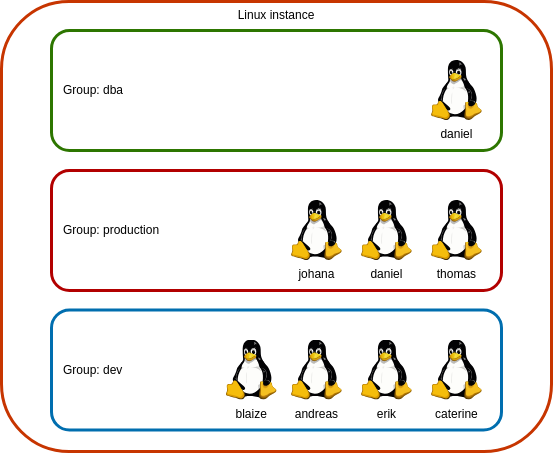
\includegraphics[width=6cm]{image/groups-and-users.drawio}
        \end{columns}
    \end{frame}

    \begin{frame}[fragile]
        \transdissolve
        \frametitle{Utilisateurs, groupes et droits d'accès}
        \framesubtitle{Les groupes}
        L'utilitaire \lstinline{addgroup} permet de créer un groupe.
%bash listing
        \begin{lstlisting}[language=bash]
$ whoami
chrichri
$ addgroup digicomp
fatal: Seul le superutilisateur est autorisé à ajouter un utilisateur ou un groupe au système.
        \end{lstlisting}
        Pourquoi cela ne fonctionne pas~?
        \pause
        \begin{dangercolorbox}
            Pour ajouter un groupe, il faut être superutilisateur.
            C'est à dire, avoir les droits \textquote{root}.
            Donc être \textquote{root}, ou utiliser \lstinline{sudo} si on est \textquote{sudoer}, \textit{i.e.}, que l'on fait partie du groupe \textquote{sudo}.
        \end{dangercolorbox}
        \begin{lstlisting}[language=bash]
$ sudo addgroup digicomp
info: Choix d'un GID dans la plage 1000 à 59999 ...
info: Ajout du groupe « digicomp » (GID 1002)...
$ groups
chrichri adm dialout cdrom sudo audio dip video plugdev lpadmin pulse lxd sambashare docker libvirt nordvpn
$ members sudo
chrichri
$ members digicomp
        \end{lstlisting}
    \end{frame}

    \begin{frame}[fragile]
        \transdissolve
        \frametitle{Utilisateurs, groupes et droits d'accès}
        \framesubtitle{Les groupes}
        \lstinline{groups} permet de lister les groupes auxquels appartient un utilisateur, mais aussi de lister tous les groupes~:
        \begin{lstlisting}[language=bash]
$ groups chrichri
chrichri : chrichri adm dialout cdrom sudo audio dip video plugdev lpadmin pulse lxd sambashare nordvpn docker libvirt
        \end{lstlisting}
        \lstinline{members} permet de lister les membres d'un groupe.
        Il nous confirme que le groupe \lstinline{digicomp} est bien créé, il n'a pas de membres.
        \bigbreak
        Pour qu'une ressource, fichier, dossier, appartienne à un groupe, il faut que le groupe soit propriétaire de la ressource.
        Pour cela, la commande \lstinline{chown}(CHange OWNer) permet de changer le propriétaire d'une ressource.
% Shell listing
        \begin{lstlisting}[language=bash]
$ mkdir digicomp-little-secret
$ touch digicomp-little-secret/secret.txt
$ echo "Le code de l'entrée est 8564" > digicomp-little-secret/secret.txt
$ cat digicomp-little-secret/secret.txt
Le code de l'entrée est 8564
$ sudo chown root:digicomp -R digicomp-little-secret/
$ ls -lha digicomp-little-secret/
total 12K
drwxrwxr-x  2 root     digicomp 4,0K août  15 16:07 .
drwxrwxr-x 10 chrichri chrichri 4,0K août  15 16:07 ..
-rw-rw-r--  1 root     digicomp   29 août  15 16:08 secret.txt
        \end{lstlisting}
    \end{frame}

    \begin{frame}[fragile]
        \transdissolve
        \frametitle{Utilisateurs, groupes et droits d'accès}
        \framesubtitle{Les groupes}
        \lstinline{sudo chown root:digicomp -R digicomp-little-secret} veut dire que le groupe propriétaire de \lstinline{digicomp-little-secret} est \lstinline{digicomp} et de manière récursive, \textit{i.e.}, pour les sous-dossiers et fichiers.
        La structure de la commande est \lstinline{chown <user>:<group> -R <path>}.
        Et il faut la aussi être \textquote{superutilisateur}, ici avec \lstinline{sudo}.
        \bigbreak
        Mais\ldots
        \begin{lstlisting}[language=bash]
$ cat digicomp-little-secret/secret.txt
Le code de l'entré est 8564
$ echo "Le code de l'entré est 2539" > digicomp-little-secret/secret.txt
bash: digicomp-little-secret/secret.txt: Permission non accordée
        \end{lstlisting}
        Qu'est-ce que cela veut dire~?
        \begin{center}
            
\includegraphics[width=2.5cm]{image/question-mark}
        \end{center}
    \end{frame}

    \subsection{Droits}\label{subsec:droits}

    \begin{frame}
        \transdissolve
        \frametitle{Utilisateurs, groupes et droits d'accès}
        \framesubtitle{Les droits\footnote{\label{rights-digitalocean}An Introduction to Linux Permissions, \url{https://www.digitalocean.com/community/tutorials/an-introduction-to-linux-permissions}}}
        \begin{dangercolorbox}
            Cela montre que des users qui ne sont pas prioritaires et qui ne font pas partie du groupe propriétaire peuvent avoir des droits.
            Par défaut ces droits sont en lecture seule, n'ont n'avons pas pu écrire dans le fichier.
        \end{dangercolorbox}
        \centering
        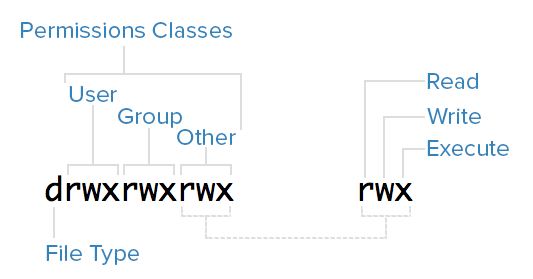
\includegraphics[width=7cm]{image/permission-classes}
        \flushleft
        Les droits par défaut du fichier en question étaient \lstinline{-rw-rw-r--}.
    \end{frame}

    \begin{frame}[fragile]
        \transdissolve
        \frametitle{Utilisateurs, groupes et droits d'accès}
        \framesubtitle{Les droits\cref{rights-digitalocean}}
        \begin{lstlisting}[language=bash]
$ ls -lha digicomp-little-secret/
total 12K
drwxrwxr-x  2 root     digicomp 4,0K août  15 16:07 .
drwxrwxr-x 10 chrichri chrichri 4,0K août  15 16:07 ..
-rw-rw-r--  1 root     digicomp   29 août  15 16:08 secret.txt
        \end{lstlisting}
        \begin{columns}
            \column{0.4\textwidth}
            N'étant ni dans le groupe propriétaire, ni propriétaire, l'utilisateur \lstinline{chrichri} est autre, ses droits sont donc \lstinline{r--}.

            Qui veut dire, \textit{read} uniquement.
            Ce qui est cohérent avec les commandes précédentes.
            \column{0.6\textwidth}
            \begin{center}
                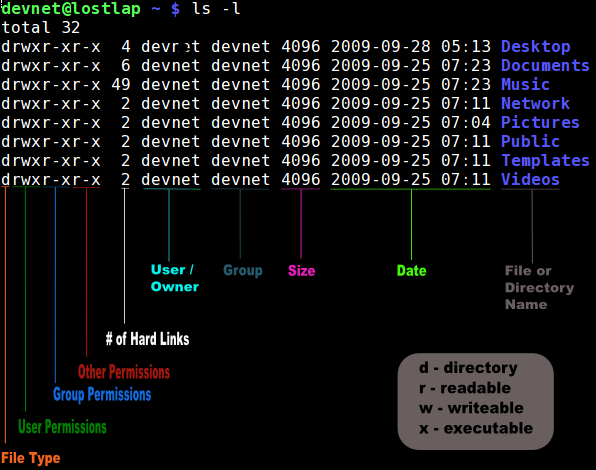
\includegraphics[width=6.5cm]{image/ls-details}
            \end{center}
        \end{columns}
    \end{frame}

    \begin{frame}
        \transdissolve
        \frametitle{Utilisateurs, groupes et droits d'accès}
        \framesubtitle{Les droits\cref{rights-digitalocean}\footnotestep\footnote{\label{octal}Octal Notation and Linux Permissions, \url{https://cratecode.com/info/octal-notation}}}
        \begin{columns}
            \column{0.5\textwidth}
            La notation octale est une manière de représenter les droits d'accès.
            \bigbreak
            \textit{In fine}, c'est un nombre qui est la concaténation de 3 suites de valeurs binaires\ldots.
            \column{0.5\textwidth}
            \begin{center}
                
\includegraphics[width=6.5cm]{image/binary-explosion}
            \end{center}
        \end{columns}
    \end{frame}

    \begin{frame}[fragile]
        \transdissolve
        \frametitle{Utilisateurs, groupes et droits d'accès}
        \framesubtitle{Représentation binaire la notation octale avec Python\cref{octal}}
        \begin{lstlisting}[language=bash]
int("000", 2) # Masque binaire de 3 de longs donc 0 est le minimum
Out[30]: 0
int("111", 2) # 7 le maximum, de 0 à 7 il y a 8 valeurs d'où octal
Out[31]: 7
int("001", 2) # Execute: --x
Out[32]: 1
int("010", 2) # Write: -w-
Out[33]: 2
int("100", 2) # Read: r--
Out[34]: 4
int("110", 2) # Read/write: rw-
Out[35]: 6
int("111", 2) # Read/write/execute: rwx
Out[36]: 7
int("011", 2) # Write/execute: -wx
Out[37]: 3
int("101", 2) # Write/execute: w-x
Out[38]: 5
        \end{lstlisting}
    \end{frame}

    \begin{frame}[fragile]
        \transdissolve
        \frametitle{Utilisateurs, groupes et droits d'accès}
        \framesubtitle{Notation octale\cref{octal}}
        Cela fait bien des droits qui vont de 0 pour la lecture seule au user, à 777 pour la lecture, l'écriture et l'exécution au user, groupe et autres.
        \begin{lstlisting}[language=bash]
"".join(map(str, [int("100", 2), int("000", 2), int("000", 2)])) # r-- pour user
Out[46]: '400'
"".join(map(str, [int("111", 2), int("111", 2), int("111", 2)])) # rwx pour tous
Out[45]: '777'
        \end{lstlisting}
        Ces droits s'appliquent avec la commande \lstinline{chmod} pour CHange MODe.
        Selon le format suivant \lstinline{chmod <mode> <file>}.
        \lstinline{<mode>} étant le chiffre calculé entre 000 et 777 calculé au dessus.
        Comme pour \lstinline{chown}, l'option \lstinline{-R} peut être ajoutée pour être récursif dans les sous-dossiers et fichiers.
        \bigbreak
        Des utilitaires plus user friendly que Python sont en ligne comme \url{https://chmod-calculator.com/}.
    \end{frame}

    \begin{frame}[fragile]
        \transdissolve
        \frametitle{Utilisateurs, groupes et droits d'accès}
        \framesubtitle{Notation octale\cref{octal}}
        En résumé, restreindre les droits à la lecture par l'utilisateur propriétaire m'empêche de lire le fichier~:
        \begin{lstlisting}[language=bash]
$ sudo chmod 400 digicomp-little-secret/secret.txt
$ cat digicomp-little-secret/secret.txt
cat: digicomp-little-secret/secret.txt: Permission non accordée
        \end{lstlisting}
        Graĉe à \lstinline{sudo} je peux me donner les droits en lecture ou écriture par exemple~:
        \begin{lstlisting}[language=bash]
$ sudo chmod 007 digicomp-little-secret/secret.txt
$ cat digicomp-little-secret/secret.txt
Le code de l'entrée est 8564
$ sudo chmod 002 digicomp-little-secret/secret.txt
$ cat digicomp-little-secret/secret.txt
cat: digicomp-little-secret/secret.txt: Permission non accordée
$ echo "Le code de l'entrée est 8564" > digicomp-little-secret/secret.txt
        \end{lstlisting}
    \end{frame}

    \subsection{Utilisateurs}\label{subsec:utilisateurs}
    \begin{frame}
        \transdissolve
        \frametitle{Utilisateurs, groupes et droits d'accès}
        \framesubtitle{Les utilisateurs}
        Les utilisateurs sont les personnes qui utilisent le système.
        Les bonnes pratiques veulent qu'il y en a un par personne physique.
        L'utilisateur a pour s'identifier un user et un mot de passe et/ou une clé privé.
        C'est l'administrateur du système qui lui génère son premier mot de passe et sa première clé.
        Un user peut faire partie de plusieurs groupes, comme ici \lstinline{daniel} qui est \lstinline{dba} et \lstinline{prod}.
        \begin{columns}
            \column{0.5\textwidth}
            Exemple de commandes pour gérer un utilisateur~:
            \begin{itemize}
                \item \lstinline{adduser}~: Ajouter un utilisateur.
                \item \lstinline{passwd}~: Changer le mot de passe.
                \item \lstinline{usermod}~: Modifier un utilisateur.
                \item \lstinline{userdel}~: Supprimer un utilisateur.
            \end{itemize}
            \column{0.5\textwidth}
            \centering
            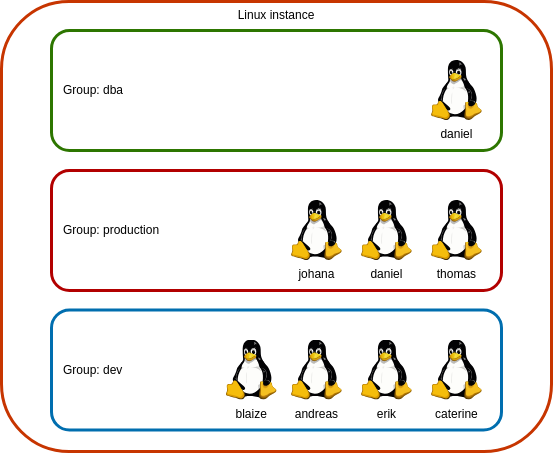
\includegraphics[width=5cm]{image/groups-and-users.drawio}
        \end{columns}
    \end{frame}

    \begin{frame}[fragile]
        \transdissolve
        \frametitle{Utilisateurs, groupes et droits d'accès}
        \framesubtitle{Les utilisateurs}
        Exemple avec la création du user \lstinline{digiformateur}.
        \begin{lstlisting}[language=bash]
$ useradd -s /bin/bash -m -d $/home/digiformateur digiformateur
useradd: Permission denied.
useradd : impossible de vérouiller /etc/passwd ; réessayer plus tard.
$ sudo useradd -s /bin/bash -m -d $/home/digiformateur digiformateur # sudo
$ passwd digiformateur
passwd : Vous ne devriez pas voir ou modifier l'information du mot de passe pour digiformateur.
$ sudo passwd digiformateur # superutilisateur
Nouveau mot de passe : 
Retapez le nouveau mot de passe : 
passwd : mot de passe mis à jour avec succès
$ su digiformateur
Mot de passe : 
$ whoami
digiformateur
$ exit
exit
$ userdel digiformateur # superutilisateur
userdel: Permission denied.
userdel : impossible de vérouiller /etc/passwd ; réessayer plus tard.
$ sudo userdel digiformateur
        \end{lstlisting}
    \end{frame}

    \subsection{Mot de passe}\label{subsec:password}
    \begin{frame}
        \transdissolve
        \frametitle{Utilisateurs, groupes et droits d'accès}
        \framesubtitle{Recommandation sur les motrs de passe}
        \begin{footnotesize}
            Bonnes pratiques de l'ANSSI\footnote{Bonnes pratiques - Protégez-vous !, \url{https://cyber.gouv.fr/bonnes-pratiques-protegez-vous}} pour les mots de passe~:
            \begin{columns}
                \column{0.5\textwidth}
                \begin{itemize}
                    \item Créez un mot de passe suffisamment long, complexe et inattendu :
                    de 8 caractères minimum et contenant des minuscules, des majuscules,
                    des chiffres et des caractères spéciaux.

                    \item Ne communiquez jamais votre mot de passe à un tiers : aucune
                    organisation ou personne de confiance ne vous demandera de lui
                    communiquer votre mot de passe.

                \end{itemize}
                \column{0.6\textwidth}
                \centering
                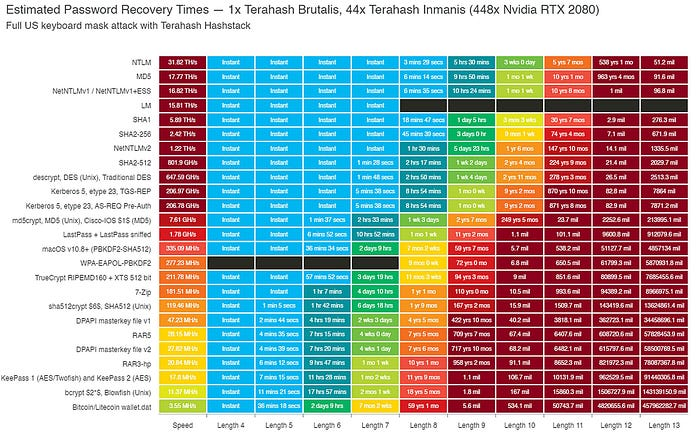
\includegraphics[width=6.5cm]{image/real-password-cracking} \\ Hashcat benchmark\footnotemark \\
            \end{columns}
            Mais le mot de passe seul n'est pas suffisant, le plus sûr reste le SSH avec la pair de clés privé et publique.
            \footnotetext{Those Tables With Password Cracking Times That Scare You And Peddle Snake Oil — Are Mostly Wrong!, \url{https://billatnapier.medium.com/those-tables-password-cracking-times-that-scare-you-are-mostly-wrong-7d03bf4aec6}}
        \end{footnotesize}
    \end{frame}

    \subsection{Exercice}\label{subsec:user-group-rights-exercice}
    \begin{frame}
        \transdissolve
        \frametitle{Utilisateurs, groupes et droits d'accès}
        \framesubtitle{Exercice \execcounterdispinc}
        Cet exercice a pour objectif de montrer que les droits d'accès sont une question de sécurité, les configurations et les services sont très sensibles.
        En effet, les services sont le plus exécutés par l'utilisateur root et ont donc le maximum de droits.
        \bigbreak
        Il est courant de donner des droits en lecture seule à un fichier de configuration, mais de ne pas donner de droits en écriture.
        \begin{itemize}
            \item Créer un user qui aura des droits en écriture sur la configuration d'un service dans \lstinline{/etc/systemd/system}.
            \item Créer un groupe qui aura des droits en écriture sur la configuration d'un autre service dans \lstinline{/etc/systemd/system}.
            \item Ajouter à ce dernier groupe le nouveau user.
            \item Supprimer groupe et user.
            \item Remettre les droits comme avant sur les deux services.
        \end{itemize}
    \end{frame}

    \begin{frame}
        \transdissolve
        \frametitle{Utilisateurs, groupes et droits d'accès}
        \framesubtitle{Exercice \execcounterdispinc}
        Cet exercice a pour objectif de créer un simple site web static isolé par le jeu des user/groupes/droits.
        \begin{itemize}
            \item Créer un groupe pour ce serveur/site web.
            \item Créer un user type développeur qui aura des droits adéquats sur un dossier et fichier \lstinline{/var/www/html/digicomp/index.html}.
            \item Créer un user type production qui aura des droits adéquats sur un dossier et fichier \lstinline{/var/www/html/digicomp/index.html}.
            \item Un script shell à exécuter grâce au shebang \lstinline{\#!/bin/bash} qui lance la commande Python \lstinline{python3 -m http.server -d /var/www/html/digicomp/}.
            Ce script shell ne peut être exécuté par l'utilisateur de production uniquement et aucune resource ne doit pouvoir être modifiée.
        \end{itemize}
    \end{frame}


    \section{Système de fichiers}\label{sec:fs}
    \begin{frame}
        \transdissolve
        \frametitle{Système de fichiers}
        \framesubtitle{Définition\footnote{\label{fs}Les systèmes de fichiers sous GNU-Linux / macOS / Windows, \url{https://doc.ubuntu-fr.org/systeme_de_fichiers}}}
        \begin{footnotesize}
            Soft qui organise les fichiers de votre ordinateur sur votre disque dur de façon
            à pouvoir les retrouver lorsque vous au besoin.
            Les systèmes de fichiers les plus répandus à l'heure actuelle sont sûrement le FAT32 et
            le NTFS, qui sont les deux seuls systèmes de fichiers que Microsoft® Windows® peut nativement lire.
            Il existe de nombreux autres systèmes de fichiers : ext2, ext3, ext4, ReiserFS, JFS, XFS, Btrfs, ZFS\ldots
            \begin{table}[h!]
                \centering
                \begin{tabular}{|c|c|c|c|c|}
                    \hline
                    \textbf{Nom} & \textbf{Fichier max} & \textbf{Partition max} & \textbf{Journalisé} & \textbf{Gestion des droits} \\ \hline
                    BtrFS        & 16 EiB               & 16 EiB                 & Non (CoW)           & Oui                         \\ \hline
                    exFAT        & 16 TiB               & 256 TiB                & Oui                 & Oui                         \\ \hline
                    ext2FS       & 2 TiB                & 4 TiB                  & Non                 & Oui                         \\ \hline
                    ext3FS       & 2 TiB                & 4 TiB                  & Oui                 & Oui                         \\ \hline
                    ext4FS       & 16 TiB               & 1 EiB                  & Oui                 & Oui                         \\ \hline
                    FAT          & 2 GiB                & 2 GiB                  & Non                 & Non                         \\ \hline
                    FAT32        & 4 GiB                & 8 TiB                  & Non                 & Non                         \\ \hline
                    NTFS         & 16 TiB               & 256 TiB                & Oui                 & Oui                         \\ \hline
                    ReiserFS     & 8 TiB                & 16 TiB                 & Oui                 & Oui                         \\ \hline
                    UDF          & 16 EiB               & 2 To                   & Non                 & Oui                         \\ \hline
                \end{tabular}
            \end{table}
        \end{footnotesize}
    \end{frame}

    \begin{frame}[fragile]
        \transdissolve
        \frametitle{Système de fichiers}
        \framesubtitle{Définition\cref{fs}}
        Sans cette indexation, il serait impossible de retrouver un fichier sur un disque dur.
        Qui n'est que une immensité de données binaire~:
        \begin{lstlisting}
$ sudo dd if=/dev/nvme0n1p3 ibs=512 count=1 skip=239 2> /dev/null | hexdump -C
00000000  00 d7 01 d7 02 d7 03 d7  04 d7 05 d7 06 d7 07 d7  |................|
00000010  08 d7 09 d7 0a d7 0b d7  0c d7 0d d7 0e d7 0f d7  |................|
00000020  10 d7 11 d7 12 d7 13 d7  14 d7 15 d7 16 d7 17 d7  |................|
00000030  18 d7 19 d7 1a d7 1b d7  1c d7 1d d7 1e d7 1f d7  |................|
00000040  20 d7 21 d7 22 d7 23 d7  24 d7 25 d7 26 d7 27 d7  | .!.".#.$.%.&.'.|
00000050  28 d7 29 d7 2a d7 2b d7  2c d7 2d d7 2e d7 2f d7  |(.).*.+.,.-.../.|
00000060  30 d7 31 d7 32 d7 33 d7  34 d7 35 d7 36 d7 37 d7  |0.1.2.3.4.5.6.7.|
00000070  38 d7 39 d7 3a d7 3b d7  3c d7 3d d7 3e d7 3f d7  |8.9.:.;.<.=.>.?.|
        \end{lstlisting}
        \lstinline{dd} est une commande qui permet de lire et écrire des tout ou partie d'un disque
        \bigbreak
        Par défaut sur les machine Ubuntu le système de fichier est \lstinline{ext4}.
        \bigbreak
        Mais ZFS est aussi supporté.
        Il est plus courant sur les serveurs qui stock des données, plus que sur les serveurs applicatif.
    \end{frame}

    \begin{frame}
        \transdissolve
        \frametitle{Système de fichiers}
        \framesubtitle{Du hardware au Kernel\footnote{Linux File System\url{https://www.javatpoint.com/linux-file-system}}}
        \centering
        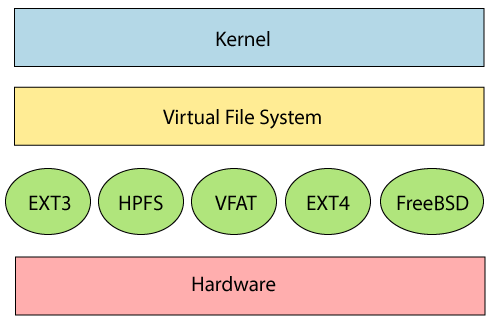
\includegraphics[width=11cm]{image/linux-file-system-stack}
    \end{frame}

    \subsection{Montage du système de fichiers}\label{subsec:mount}
    \begin{frame}[fragile]
        \transdissolve
        \frametitle{Système de fichiers}
        \framesubtitle{Comment rajouter un disque~?}
        \begin{scriptsize}
            \begin{itemize}
                \item \lstinline{lsblk}~: Pour lister les disques et les partitions.
                \item \lstinline{parted}~: Pour lister et modifier les disques et les partitions.
                \item \lstinline{mount}~: Pour monter le disque.
                \item \lstinline{df}~: Pour vérifier que le disque est bien monté.
            \end{itemize}
            \begin{lstlisting}[language=bash,basicstyle=\tiny\ttfamily]
$ sudo parted -l
Modèle : KPART512GBC2DVT (nvme)
Disque /dev/nvme0n1 : 512GB
Taille des secteurs (logiques/physiques) : 512B/512B
Table de partitions : gpt
Drapeaux de disque :

Numéro  Début   Fin    Taille  Système de fichiers  Nom                           Drapeaux
 1      1049kB  211MB  210MB   fat32                EFI system partition          démarrage, esp
 2      211MB   228MB  16,8MB                       Microsoft reserved partition  msftres
 3      228MB   129GB  129GB   ntfs                 Basic data partition          msftdata
 4      129GB   233GB  104GB   ntfs                 Basic data partition          msftdata
 8      233GB   491GB  258GB   ext4


Modèle : Inconnu (unknown)
Disque /dev/zram0 : 8271MB
Taille des secteurs (logiques/physiques) : 4096B/4096B
Table de partitions : loop
Drapeaux de disque :

Numéro  Début  Fin     Taille  Système de fichiers  Drapeaux
 1      0,00B  8271MB  8271MB  linux-swap(v1)
            \end{lstlisting}
        \end{scriptsize}
    \end{frame}

    \begin{frame}
        \transdissolve
        \frametitle{Système de fichiers}
        \framesubtitle{Comment rajouter un disque~?}
        Combien de disque physique~?
        \begin{center}
            
\includegraphics[width=3cm]{image/question-mark}
        \end{center}
        \pause
        \begin{dangercolorbox}
            Il y a un seul disque(s) physique(s), \lstinline{/dev/nvme0n1}.

            L'autre est la RAM, une partie du système de fichier, celle dédiée au fichiers temporaires est mappée sur la RAM pour des soucis de performance.
        \end{dangercolorbox}
    \end{frame}

    \begin{frame}[fragile]
        \transdissolve
        \frametitle{Système de fichiers}
        \framesubtitle{Comment rajouter un disque~?}
        \begin{scriptsize}
            En connectant un nouveau disque on constate bien avec \lstinline{parted} qu'il y a un nouveau disque~:
            \begin{lstlisting}[language=bash,basicstyle=\tiny\ttfamily]
Modèle : Intuix DiskOnKey (scsi)
Disque /dev/sda : 252MB
Taille des secteurs (logiques/physiques) : 512B/512B
Table de partitions : loop
Drapeaux de disque :

Numéro  Début  Fin    Taille  Système de fichiers  Drapeaux
 1      0,00B  252MB  252MB   ext4
            \end{lstlisting}
            4 To environ au format NTFS, il est sous \lstinline{/dev/sda}.
            A-t-il un point de montage sur le système de fichier~?
            \begin{lstlisting}[language=bash,basicstyle=\tiny\ttfamily]
$ df
Sys. de fichiers        blocs de 1K   Utilisé Disponible Uti% Monté sur
tmpfs                       1615420      6264    1609156   1% /run
/dev/nvme0n1p8            247090272 199514156   34951836  86% /
tmpfs                       8077096     11248    8065848   1% /dev/shm
tmpfs                          5120         8       5112   1% /run/lock
efivarfs                        184       172          8  96% /sys/firmware/efi/efivars
tmpfs                       8077096         0    8077096   0% /run/qemu
tmpfs                       2097152      3400    2093752   1% /tmp
/dev/nvme0n1p1               200704     51428     149276  26% /boot/efi
tmpfs                       1615416      2596    1612820   1% /run/user/1000
/home/chrichri/.Private   247090272 199514156   34951836  86% /home/chrichri/Private
            \end{lstlisting}
        \end{scriptsize}
    \end{frame}

    \begin{frame}[fragile]
        \transdissolve
        \frametitle{Système de fichiers}
        \framesubtitle{Comment rajouter un disque~?}
        Créons un \textquote{point de montage} et montons ce disque~:
        \begin{lstlisting}[language=bash]
$ sudo mkdir /mnt/sda-usb # /mnt pour les montage par convention mais peut être ailleurs
$ sudo mkfs.ext4 /dev/sda # formatage du disque en Ext4 car le FS était incompatible
$ sudo mount /dev/sda /mnt/sda-usb
$ ls /mnt/sda-usb -lha
total 24K
drwxr-xr-x 3 root root 4,0K août  17 15:21 .
drwxr-xr-x 5 root root 4,0K août  17 15:08 ..
drwx------ 2 root root  16K août  17 15:21 lost+found
        \end{lstlisting}
        \begin{dangercolorbox}
            \lstinline{mkfs.ext4} est une commande qui permet de formater un disque en Ext4.
            Elle supprime donc les données du disque.
            Elle est néanmoins nécessaire pour pouvoir monter le disque, il y avait en effet une incompatibilité de système de fichier.
            Ces incompatibilités sont fréquentes avec les systèmes de fichiers Windows® comme FAT et NTFS~.
        \end{dangercolorbox}
    \end{frame}

    \begin{frame}[fragile]
        \transdissolve
        \frametitle{Système de fichiers}
        \framesubtitle{Comment rajouter un disque~?}
        Comme ces commandes ont été exécutées par le supersaturation, il est probable ques les droits bloque l'écriture~:
        \begin{lstlisting}[language=bash]
$ cp ocr_speed.txt /mnt/sda-usb
cp: impossible de créer le fichier standard '/mnt/sda-usb/ocr_speed.txt': Permission non accordée
$ sudo cp ocr_speed.txt /mnt/sda-usb
$ sudo chown chrichri: -R /mnt/sda-usb
$ sudo chmod 700 /mnt/sda-usb
$ cp ocr_speed.txt /mnt/sda-usb
$ /mnt/sda-usb/ocr_speed.txt -lha
-rw-r--r-- 1 chrichri chrichri 212 août  17 15:37 /mnt/sda-usb/ocr_speed.txt
        \end{lstlisting}
        Des modifications ont pu être apportées.
        \bigbreak
        Avant de retirer le disque peut démonter le disque et éventuellement supprimer le point de montage~:
        \begin{lstlisting}[language=bash]
$ sudo umount /dev/sda
$ ls /mnt/sda-usb
$ sudo rm -rf /mnt/sda-usb
        \end{lstlisting}
    \end{frame}

    \begin{frame}
        \transdissolve
        \frametitle{Système de fichier}
        \framesubtitle{Exercice \execcounterdispinc}
        \newcounter{exemountcounter}
        \setcounter{exemountcounter}{\value{execounter}}
        % add one as execounter not incremented yet
        \addtocounter{exemountcounter}{1}
        Cet exercice a pour objectif d'ajouter un disque en lecture seule sur votre Bureau.
        \begin{itemize}
            \item Le disque est une clé USB pluggée à votre PC~.
            \item Créer le point de montage sur le bureau.
            \item Montez-y la clé USB~.
            Après l'avoir démonter si elle a été montée automatiquement par l'OS~.
            \item Modifier les droits pour qu'elle soit en lecture seule.
            \item Démonter la clé USB~.
            \item Supprimer le point de montage.
        \end{itemize}
        \bigbreak
        \centering
        
\includegraphics[width=3cm]{image/guy-in-front-of-desktop}
    \end{frame}

    \subsection{La table du système de fichiers (/etc/fstab)}\label{subsec:fstab}
    \begin{frame}[fragile]
        \transdissolve
        \frametitle{Système de fichiers}
        \framesubtitle{La table du système de fichiers (\lstinline{/etc/fstab})}
        \lstinline{/etc/fstab} est un fichier de configuration associe des points de montage à des disques.
        Il est lu au démarrage du système pour monter les disques automatiquement et ne pas avoir à passer les commandes vues précédemment.
        \bigbreak
        Il permet également de configurer des partitions spécialisées comme \lstinline{/tmp} ou \lstinline{swapfile}.
        \begin{lstlisting}[language=bash,basicstyle=\tiny\ttfamily]
$ cat /etc/fstab
# /etc/fstab: static file system information.
#
# Use 'blkid' to print the universally unique identifier for a
# device; this may be used with UUID= as a more robust way to name devices
# that works even if disks are added and removed. See fstab(5).
#
# <file system> <mount point>   <type>  <options>       <dump>  <pass>
# / was on /dev/nvme0n1p8 during installation
UUID=9bcc82ee-9214-4eac-90f6-9695c585874b /               ext4    errors=remount-ro 0       1
# /boot/efi was on /dev/nvme0n1p1 during installation
UUID=EE30-267D  /boot/efi       vfat    umask=0077      0       1
#/swapfile                                 none            swap    sw              0       0
# Temp file in memory.
tmpfs /tmp tmpfs defaults,size=2G 0 0
        \end{lstlisting}
    \end{frame}

    \begin{frame}[fragile]
        \transdissolve
        \frametitle{Système de fichiers}
        \framesubtitle{La table du système de fichiers (\lstinline{/etc/fstab})}
        \lstinline{/etc/fstab} est un fichier de configuration associe des points de montage à des disques.
        On y trouve les UUID des disques, le point de montage, le type de système de fichier, les options de montage du disque principale~:
        \begin{lstlisting}[language=bash,basicstyle=\tiny\ttfamily]
UUID=9bcc82ee-9214-4eac-90f6-9695c585874b /               ext4    errors=remount-ro 0       1
        \end{lstlisting}
        La partition de boot montée sur \lstinline{/boot/efi}~:
        \begin{lstlisting}[language=bash,basicstyle=\tiny\ttfamily]
UUID=EE30-267D  /boot/efi       vfat    umask=0077      0       1
        \end{lstlisting}
        La \lstinline{swapfile} qui est commentée pour car c'est une extension de la RAM sur le disque, c'est configuration invite l'OS à utiliser un maximum la RAM~.
        La partition \lstinline{/tmp} montée en mémoire pour de meilleurs performances avec certaines commandes comme \lstinline{sort}, la mémoire est plus rapide que le SSD.~:
        \begin{lstlisting}[language=bash,basicstyle=\tiny\ttfamily]
# Temp file in memory.
tmpfs /tmp tmpfs defaults,size=2G 0 0
        \end{lstlisting}
        On peut aussi utiliser ce fichier pour configurer le montage au moment du démarrage d'un disque supplémentaire, clé USB sur un point de montage~:
        \begin{lstlisting}[language=bash,basicstyle=\tiny\ttfamily]
# /boot was on /dev/sda5 during installation
/dev/sda5                                    /boot           ext2    defaults          0       2
        \end{lstlisting}
    \end{frame}

    \begin{frame}
        \transdissolve
        \frametitle{Système de fichiers}
        \framesubtitle{Exercices de configuration de la table du système de fichiers (\lstinline{/etc/fstab})}
        Exercice \execcounterdispinc: Reprendre les consignes de l'exercice  \theexemountcounter{} et ajouter le disque à la table du système de fichiers \lstinline{/etc/fstab} pour que la clé soit montée automatiquement au démarrage.
        \bigbreak
        Exercice \execcounterdispinc: Créer un disque virtuel de 1 Go et le monter automatiquement au démarrage en configurant \lstinline{/etc/fstab}.
        \bigbreak
        \centering
        
\includegraphics[width=3cm]{image/guy-in-front-of-desktop}
    \end{frame}

    \subsection{RAID)}\label{subsec:raid}

    \begin{frame}
        \transdissolve
        \frametitle{RAID}
        \framesubtitle{Les différents RAID\footnote{\label{mdadm}mdadm : RAID Logiciel sous Linux, \url{https://www.linuxtricks.fr/wiki/mdadm-raid-logiciel-sous-linux}}\footnotestep\footnote{Qu'est-ce que le RAID ?, \url{https://www.diskpart.com/fr/windows-server/logiciel-gestion-raid-8899-tc.html}}}
        Le RAID est un ensemble de standards de virtualisation du stockage permettant de répartir des données sur plusieurs disques durs afin d'améliorer soit les performances, soit la sécurité ou la tolérance aux pannes de l'ensemble du ou des systèmes.
        \bigbreak
        \centering
        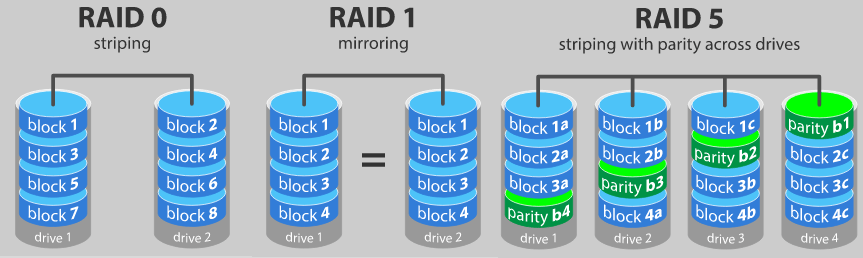
\includegraphics[width=10cm]{image/raid-0-1-5} \\ Les principaux RAID, les 0, 1 et 5 \\
    \end{frame}

    \begin{frame}
        \transdissolve
        \frametitle{RAID}
        \framesubtitle{\lstinline{mdadm}\cref{mdadm}\footnotestep\footnote{RAID logiciel avec mdadm, \url{https://doc.ubuntu-fr.org/raid_logiciel}}}
        \begin{itemize}
            \item Logiciel installable sous Ubuntu avec le package manager, pas besoin de compilation.
            \item Comme pour les autres commandes \textquote{bas-niveau}, elle nécessite d'être superutilisateur.
            \item Il lance un service qui monitor les processus nécessaires au RAID~.
            Un service se lance automatiquement au démarrage du système.
            \item Il faut que les disques soient vierges, sinon les données seront perdues.
            \item Il est recommandé qu'ils aient la même taille, mais ce n'est pas indispensable.
            Dans le cas contraire, l'espace dédié au RAID sera de la taille du plus petit disque et le reste sera non-RAID~.
            \item Ajout de disques dit \textquote{spare} ou en français dormants, qui ne sont pas utilisés par le RAID tant qu'un autre disque n'est pas tombé en panne.
        \end{itemize}
    \end{frame}

    \begin{frame}
        \transdissolve
        \frametitle{RAID}
        \framesubtitle{RAID logiciel ou controller RAID hardware?}
        \begin{itemize}
            \item Le RAID logiciel est plus flexible, car il est indépendant du matériel.
            Surtout si le controller n'est une carte du type PCIe mais qu'il est intégré à la carte mère.
            \item Le RAID hardware est plus performant, car il est géré par un processeur dédié.
            Le software prend des ressources qui pourraient être utilisées par d'autres softwares.
            \item Le RAID hardware est plus cher, car il nécessite un contrôleur RAID~.
            \item Le RAID hardware est plus difficile à maintenir.
            \item Un Contrôleurs RAID Intel® coûtent 100 à 700 CHF~.
        \end{itemize}
    \end{frame}

    \begin{frame}
        \transdissolve
        \frametitle{RAID}
        \framesubtitle{Exercice \execcounterdispinc{}}
        L'objectif est de maîtriser les commandes de base de l'outil \lstinline{mdadm}\cref{mdadm}.
        \begin{itemize}
            \item Créer 2 disques vierges de 1 Go chacun.
            \item Lancer la VM Ubuntu avec les 2 disques créés.
            \item Se connecter à la VM~.
            \item Vérifier l'ajout des 2 disques avec une commande vue précédemment.
            \item Suivre le tutorial \url{https://www.linuxtricks.fr/wiki/mdadm-raid-logiciel-sous-linux} pour créer un RAID 1.
        \end{itemize}
        \bigbreak
        \centering
        
\includegraphics[width=3cm]{image/guy-in-front-of-desktop}
    \end{frame}

    \begin{frame}
        \transdissolve
        \frametitle{RAID}
        \framesubtitle{Exercice \execcounterdispinc{}}
        Quel est un des dangers de RAID 0?
        \bigbreak
        \centering
        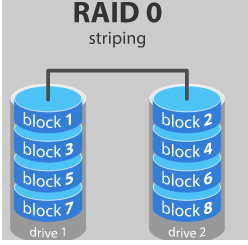
\includegraphics[width=5cm]{image/raid-0}
    \end{frame}

    \subsection{LVM)}\label{subsec:lvm}

    \begin{frame}
        \transdissolve
        \frametitle{Logical Volume Manager, A.K.A LVM}
        \framesubtitle{Définition\footnote{\label{lvm}LVM, une autre manière de partitionner, \url{https://doc.ubuntu-fr.org/lvm}}}
        Il permet la création et la création de volumes logiques.
        Ces derniers sont des partitions virtuelles qui peuvent être agrandies ou réduites sans perte de données.
        Et sont décorrélées des disques physiques (les PV ou \textquote{Physical Volume}).
        \bigbreak
        Un ou plusieurs PV sont regroupés en un ou plusieurs VG \textquote{Volume group}.
        \bigbreak
        C'est dans ces VG que sont créés les LV \textquote{Logical Volume} qui remplacent les partitions.
        \bigbreak
        Un des bénéfices est qu'un dossier comme par exemple \lstinline{/var/lib/mysql} qui contient les données de la base MySQL peut être plus grand qu'un disque physique entier~!
    \end{frame}

    \begin{frame}
        \transdissolve
        \frametitle{Logical Volume Manager, A.K.A LVM}
        \framesubtitle{Définition\cref{lvm}}
        \centering
        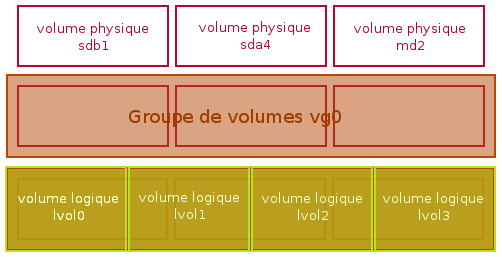
\includegraphics[width=10cm]{image/lvm}
        \flushleft
        Le PV peut être un disque RAID, par sécurité, pour prévenir une perte de données c'est même conseillé.
    \end{frame}

    \begin{frame}
        \transdissolve
        \frametitle{Logical Volume Manager, A.K.A LVM}
        \framesubtitle{Définition\cref{lvm}}
        Si les données sont strippées (avec les options \lstinline{-I} et/ou \lstinline{-i} de \lstinline{lvm2}\footnote{Analysing a Standard Logical Volume, \url{https://www.theurbanpenguin.com/striped-lvm-volumes/}}) le risque de perte de données est plus grand sans RAID mais la performance est meilleure comme avec RAID 0.
        \bigbreak
        \begin{columns}
            \column{0.5\textwidth}
            L'idéale en terme de sécurité et de performance est d'avoir un RAID 1 pour les PV et les volumes logiques strippées.
            \bigbreak
            Par défaut, avec la commande \lstinline{mount}, le montage configuré sera perdu au redémarrage.
            Une configuration de \lstinline{/etc/fstab} permet de garder le montage du LV après redémarrage.
            \column{0.5\textwidth}
            \bigbreak
            \centering
            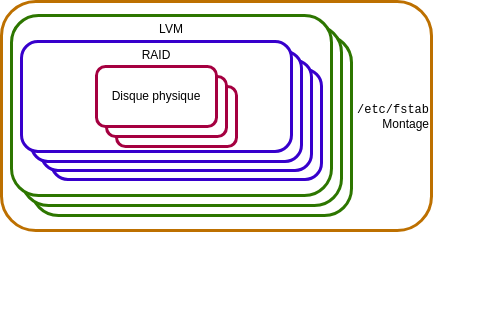
\includegraphics[width=7cm]{image/fs-stack.drawio}
        \end{columns}
    \end{frame}

    \begin{frame}
        \transdissolve
        \frametitle{Système de fichier}
        \framesubtitle{Exercice \execcounterdispinc}
        Avec le disque RAID créé précédemment, il est possible de créer un volume logique avec LVM~.
        \begin{itemize}
            \item Créer un volume physique~.
            \item Créer un groupe logique~.
            \item Créer un volume logique~.
            \item Monter le volume logique sur \lstinline{/lib/var/mysql}.
            \item Ajouter le montage du volume logique dans \lstinline{/etc/fstab} pour que le volume se monte au démarrage de la machine.
            \item Redémarrer la machine pour tester.
        \end{itemize}
    \end{frame}


    \section{Processus}\label{sec:processus}

    \subsection{Gestion des processus}\label{subsec:process-management}

    \begin{frame}
        \transdissolve
        \frametitle{Gestion des processus}
        \framesubtitle{Définition\footnote{\label{process}Les processus sous Linux, \url{https://www.cyberciti.biz/faq/how-to-check-running-process-in-ubuntu-linux-using-command-line/}}}
        Un processus est un programme en cours d'exécution.
        Il est identifié par un PID, le \textquote{Process IDentifier}.
        \bigbreak
        Il peut être en cours d'exécution, en attente, en pause, en zombie, dormant ou en terminaison, \textit{etc}.
        Il est possible de voir les processus avec la commande \lstinline{ps} ou \lstinline{top}.
        \bigbreak
        \begin{columns}
            \column{0.7\textwidth}
            \lstinline{ps} affiche les informations de manière statique alors que est dynamique, interactif et temps réel.
            \lstinline{ps} peut donc être utilisé également dans des scripts Shell.

            Les processus peuvent être tués avec la commande \lstinline{kill}.

            Les données les concernant sont stockées dans le dossier \lstinline{/proc}.
            \column{0.3\textwidth}
            \centering
            
\includegraphics[width=4cm]{image/proc-hamster}
        \end{columns}
    \end{frame}

    \begin{frame}[fragile]
        \transdissolve
        \frametitle{Gestion des processus}
        \framesubtitle{Les commandes \lstinline{ps}}
        L'option \lstinline{-f} affiche plus d'informations sur les processus.
        \begin{lstlisting}[language=bash,basicstyle=\tiny\ttfamily]
$ ps
    PID TTY          TIME CMD
 276321 pts/5    00:00:00 bash
 338450 pts/5    00:00:00 ps
$ ps -f
UID          PID    PPID  C STIME TTY          TIME CMD
chrichri  276321  265707  0 13:17 pts/5    00:00:00 /usr/bin/bash --rcfile /home/chrichri/pycharm-professional-2024.1.4/pycharm-2024.1.4/plugins/terminal/shell-integrations/bash/bash-integration.bash -i
chrichri  338508  276321 99 14:12 pts/5    00:00:00 ps -f
        \end{lstlisting}
        Une commande par nom de processus et avec la ligne de commande complète~:
        \begin{lstlisting}[language=bash,basicstyle=\tiny\ttfamily]
$ ps -fC java
UID          PID    PPID  C STIME TTY          TIME CMD
chrichri  265707    8404 80 13:08 ?        00:42:46 /home/chrichri/pycharm...
        \end{lstlisting}
        \bigbreak
        Les processus de l'utilisateur courant~:
        \begin{lstlisting}[language=bash,basicstyle=\tiny\ttfamily]
$ ps -u chrichri
    PID TTY          TIME CMD
   8059 ?        00:00:06 systemd
   8068 ?        00:00:00 (sd-pam)
   8090 ?        00:00:02 pipewire
...
        \end{lstlisting}
        \bigbreak
        Les processus de l'utilisateur courant et de tous les autres utilisateurs, \textit{i.e.}, tous les processus~:
        \begin{lstlisting}[language=bash,basicstyle=\tiny\ttfamily]
$ ps -ef
UID          PID    PPID  C STIME TTY          TIME CMD
root           1       0  0 09:23 ?        00:00:05 /sbin/init splash
root           2       0  0 09:23 ?        00:00:00 [kthreadd]
...
        \end{lstlisting}
    \end{frame}

    \begin{frame}
        \transdissolve
        \frametitle{Gestion des processus}
        \framesubtitle{Les états d'un processus sous \lstinline{ps}}
        \begin{table}[h!]
            \centering
            \begin{tabular}{|p{0.1\textwidth}|p{0.8\textwidth}|}
                \hline
                \textbf{État} & \textbf{Description}                                                            \\ \hline
                \textbf{D}    & Sommeil ininterrompu (habituellement en attente d'IO)                           \\ \hline
                \textbf{R}    & En cours d'exécution ou prêt à être exécuté (dans la file d'attente)            \\ \hline
                \textbf{S}    & Sommeil interrompible (en attente de la complétion d'un événement)              \\ \hline
                \textbf{T}    & Arrêté, soit par un signal de contrôle de tâche, soit parce qu'il est tracé     \\ \hline
                \textbf{W}    & Pagination (non valide depuis le noyau 2.6.xx)                                  \\ \hline
                \textbf{X}    & Mort (ne devrait jamais être vu)                                                \\ \hline
                \textbf{Z}    & Processus défunt ("zombie"), terminé mais non récupéré par son processus parent \\ \hline
            \end{tabular}
            \caption{États des processus sous Linux sous \lstinline{ps}}
        \end{table}
    \end{frame}

    \begin{frame}
        \transdissolve
        \frametitle{Gestion des processus}
        \framesubtitle{L'interface \lstinline{top}}
        La commande \lstinline{top} affiche tous les processus.
        Mais il ne permet pas de trouver les processus par nom contrairement à \lstinline{ps}.
        \bigbreak
        Les principales fonctions que l'on peut appeler dans l'interface~:
        \begin{table}[h!]
            \centering
            \begin{tabular}{|p{0.1\textwidth}|p{0.8\textwidth}|}
                \hline
                \textbf{Touche} & \textbf{Fonction}                           \\ \hline
                \textbf{k}      & Met fin à un processus                      \\ \hline
                \textbf{m}      & Trie la liste par utilisation de la mémoire \\ \hline
                \textbf{n}      & Trie la liste par PID                       \\ \hline
                \textbf{r}      & Modifie la priorité d’un processus          \\ \hline
                \textbf{h}      & Affiche la fenêtre d’aide                   \\ \hline
                \textbf{z}      & Affiche les processus en cours en couleurs  \\ \hline
                \textbf{d}      & Modifie l’intervalle de rafraîchissement    \\ \hline
                \textbf{c}      & Affiche le chemin absolu d’un processus     \\ \hline
                \textbf{f}      & Écran de personnalisationff                 \\ \hline
            \end{tabular}
            \caption{États des processus sous Linux sous \lstinline{top}}
        \end{table}
    \end{frame}

    \begin{frame}
        \transdissolve
        \frametitle{Gestion des processus}
        \framesubtitle{Les états d'un processus sous \lstinline{top}}
        \begin{table}[h!]
            \centering
            \begin{tabular}{|p{0.1\textwidth}|p{0.8\textwidth}|}
                \hline
                \textbf{État} & \textbf{Description}                      \\ \hline
                \textbf{D}    & Sommeil ininterrompu                      \\ \hline
                \textbf{I}    & Inactif                                   \\ \hline
                \textbf{R}    & En cours d'exécution                      \\ \hline
                \textbf{S}    & En sommeil                                \\ \hline
                \textbf{T}    & Arrêté par un signal de contrôle de tâche \\ \hline
                \textbf{t}    & Arrêté par un débogueur lors d'un traçage \\ \hline
                \textbf{Z}    & Processus zombie                          \\ \hline
            \end{tabular}
            \caption{États des processus sous Linux sous \lstinline{top}}
        \end{table}
    \end{frame}

    \begin{frame}
        \transdissolve
        \frametitle{Gestion des processus}
        \framesubtitle{L'interface \lstinline{top}}
        Top et \textquote{c} pour afficher la ligne de commande~:
        \bigbreak
        \centering
        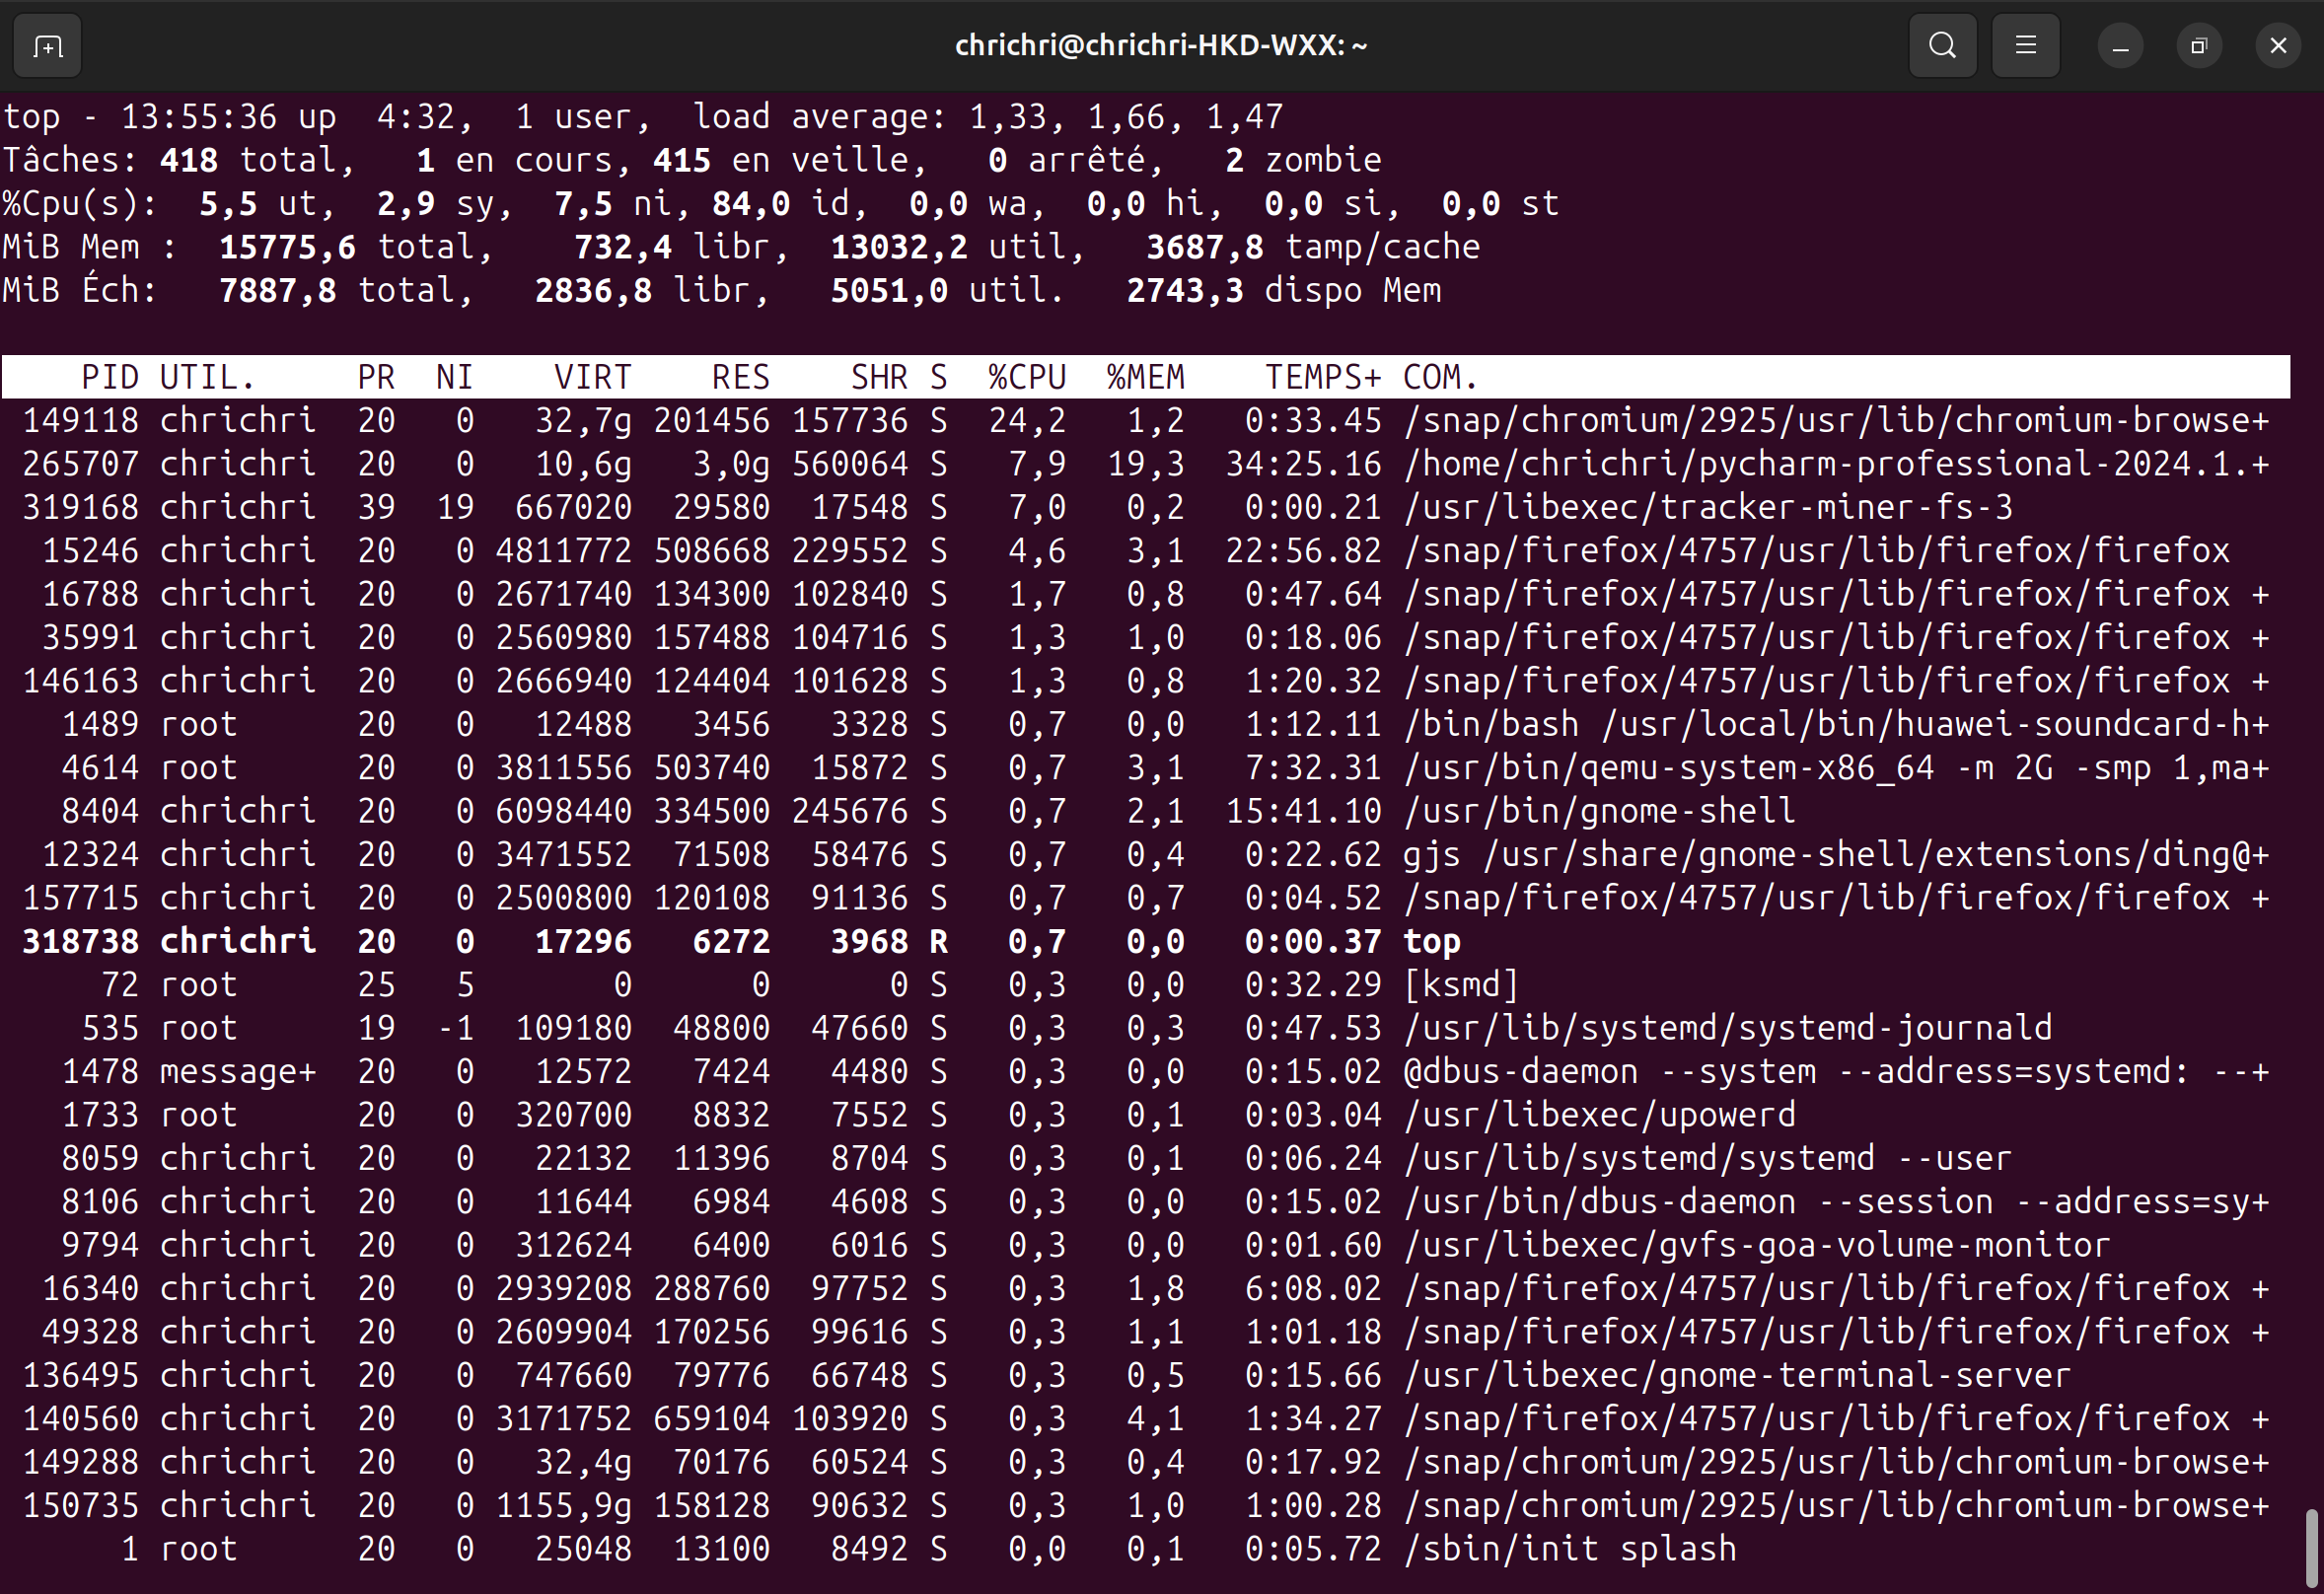
\includegraphics[width=10cm]{image/top-interface}
    \end{frame}

    \begin{frame}[fragile]
        \transdissolve
        \frametitle{Gestion des processus}
        \framesubtitle{La commande \lstinline{kill}}
        La commande \lstinline{top} permet de terminer un processus dans l'interface avec \textbf{k}.
        En fonction de son PID, qu'on aurait auparavant dans cette même interface.
        ou avec la commande \lstinline{ps}, on peut le tuer avec la commande \lstinline{kill}.
        \bigbreak
        Mais il existe une commande spécifique, c'est \lstinline{kill}.
        Elle permet de terminer un processus dont aurait trouvé le PID avec \lstinline{ps} ou \lstinline{top}.
        \begin{lstlisting}[language=bash]
$ kill -9 <PID>
        \end{lstlisting}
        \bigbreak
        La commande \lstinline{pkill} permet de tuer un processus par son nom, celui qui s'affiche dans \lstinline{ps} ou \lstinline{top}.
        \begin{lstlisting}[language=bash]
$ pkill -9 <nom>
        \end{lstlisting}
    \end{frame}

    \begin{frame}
        \transdissolve
        \frametitle{Gestion des processus}
        \framesubtitle{Le dossier \lstinline{/proc}\footnote{The /proc Filesystem, \url{https://docs.kernel.org/filesystems/proc.html}}}
        \begin{footnotesize}
            Le dossier \lstinline{/proc} contient des informations sur les processus sous l'arborescence de son PID donc \lstinline{/proc/<PID>/} dans les fichiers suivants~:
            \begin{tiny}
                \begin{table}[h!]
                    \centering
                    \begin{tabular}{|p{1.5cm}|p{9cm}|}
                        \hline
                        \textbf{File} & \textbf{Content}                                                                                                            \\
                        \hline
                        clear\_refs   & Clears page referenced bits shown in smaps output                                                                           \\
                        \hline
                        cmdline       & Command line arguments                                                                                                      \\
                        \hline
                        cpu           & Current and last cpu in which it was executed (2.4)(smp)                                                                    \\
                        \hline
                        cwd           & Link to the current working directory                                                                                       \\
                        \hline
                        environ       & Values of environment variables                                                                                             \\
                        \hline
                        exe           & Link to the executable of this process                                                                                      \\
                        \hline
                        fd            & Directory, which contains all file descriptors                                                                              \\
                        \hline
                        maps          & Memory maps to executables and library files (2.4)                                                                          \\
                        \hline
                        mem           & Memory held by this process                                                                                                 \\
                        \hline
                        root          & Link to the root directory of this process                                                                                  \\
                        \hline
                        stat          & Process status                                                                                                              \\
                        \hline
                        statm         & Process memory status information                                                                                           \\
                        \hline
                        status        & Process status in human readable form                                                                                       \\
                        \hline
                        wchan         & Present with CONFIG\_KALLSYMS=y: it shows the kernel function symbol the task is blocked in - or “0” if not blocked.        \\
                        \hline
                        pagemap       & Page table                                                                                                                  \\
                        \hline
                        stack         & Report full stack trace, enable via CONFIG\_STACKTRACE                                                                      \\
                        \hline
                        smaps         & An extension based on maps, showing the memory consumption of each mapping and flags associated with it                     \\
                        \hline
                        smaps\_rollup & Accumulated smaps stats for all mappings of the process. This can be derived from smaps, but is faster and more convenient  \\
                        \hline
                        numa\_maps    & An extension based on maps, showing the memory locality and binding policy as well as mem usage (in pages) of each mapping. \\
                        \hline
                    \end{tabular}
                \end{table}
            \end{tiny}
        \end{footnotesize}
    \end{frame}

    \begin{frame}
        \transdissolve
        \frametitle{Système de fichier}
        \framesubtitle{Exercices sur les processus}
        Exercice \execcounterdispinc{}, quels droits ai-je \lstinline{/proc} sur les processus des autres utilisateurs~?
        \bigbreak
        Exercice \execcounterdispinc{}, quels droits ai-je \lstinline{/proc} sur mes processus~?
        \bigbreak
        Exercice \execcounterdispinc{}, terminer un processus découvert sous \lstinline{top} avec la commande \lstinline{kill}.
        \bigbreak
        Exercice \execcounterdispinc{}, terminer un processus découvert sous \lstinline{top} avec la commande \lstinline{pkill}.
        \bigbreak
        Personnaliser \lstinline{top} pour que l'interface affiche les processus non pas en pourcentage totale de CPU consommé (par défaut) mais en pourcentage par coeur.
        \bigbreak
        \centering
        
\includegraphics[width=3cm]{image/guy-in-front-of-desktop}
    \end{frame}

    \begin{frame}
        \transdissolve
        \frametitle{Système de fichier}
        \framesubtitle{Exercices \execcounterdispinc{}}
        \begin{itemize}
            \item Lancer en arrière plan le script Shell \lstinline{endless-loop.sh}.
            \item Arrêter le processus correspondant au script dans \lstinline{top}.
            \item Lancer à nouveau en arrière plan le script Shell \lstinline{endless-loop.sh}.
            \item Arrêter le processus correspondant au script à l'aide de  \lstinline{ps} et \lstinline{kill}.
        \end{itemize}
        \bigbreak
        \centering
        
\includegraphics[width=3cm]{image/guy-in-front-of-desktop}
    \end{frame}

    \begin{frame}
        \transdissolve
        \frametitle{Système de fichier}
        \framesubtitle{Exercices sur les processus}
        Exercices \execcounterdispinc{}, à partir de vos connaissances sur les process et des commandes précédentes comparer l'activité d'une machine Ubuntu, d'un WSL ubuntu et d'un WSL Debian, ou un FreeBSD.

        Que remarquez-vous~?
        \pause
        \bigbreak
        \centering
        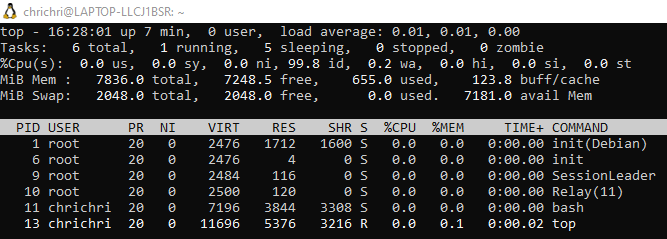
\includegraphics[width=10cm]{image/top-debian} \\ Ubuntu est-il en train de devenir un \textit{bloatware~}, lui aussi\ldots \emoji{window}?
    \end{frame}


    \section{Réseau}\label{sec:network}

    \subsection{Open SSH}\label{subsec:openssh}

    \begin{frame}{OpenSSH}{Définition\footnote{\label{openssh-site}OpenSSH, Keeping your comuniqués secret, \url{https://www.openssh.com/}}}
        \transdissolve
        OpenSSH est l'outil de connectivité principal pour les connexions à distance avec le protocole SSH.
        Il a pour but de remplacer les outils non sécurisés tels que \texttt{rlogin}, \texttt{rsh} et \texttt{telnet}.
        Il chiffre tout le trafic pour éliminer les écoutes clandestines, le détournement de connexion et d'autres attaques.
        De plus, OpenSSH offre une large gamme de capacités de tunneling sécurisé, plusieurs méthodes d'authentification et des options de configuration sophistiquées.

        La suite OpenSSH se compose des outils suivants :
        \begin{itemize}
            \item Les opérations à distance sont effectuées à l'aide de \texttt{ssh}, \texttt{scp} et \texttt{sftp}.
            \item Gestion des clés avec \texttt{ssh-add}, \texttt{ssh-keysign}, \texttt{ssh-keyscan} et \texttt{ssh-keygen}.
            \item Le côté serveur comprend \texttt{sshd}, \texttt{sftp-server} et \texttt{ssh-agent}.
        \end{itemize}
    \end{frame}

    \begin{frame}
        \transdissolve
        \frametitle{OpenSSH}
        \framesubtitle{Définition\cref{openssh-site}}
        OpenSSH est développé par quelques développeurs du projet OpenBSD et est disponible sous une licence de type BSD, donc open source.
        \bigbreak
        OpenSSH relies on the \href{https://www.libressl.org}{LibreSSL} library for some of its cryptographic routines, AES-GCM being one example.
        Plus légère que OpenSSL, LibreSSL n'a pas été affectée par des failles ayant affecté OpenSSL.
        \bigbreak
        \centering
        \includegraphics[width=7cm]{image/ssh-key-diagram}
    \end{frame}

    \begin{frame}
        \transdissolve
        \frametitle{OpenSSH}
        \framesubtitle{Les formats de clé\footnote{AUTHORIZED\_KEYS FILE FORMAT, \url{https://man.openbsd.org/sshd\#AUTHORIZED_KEYS_FILE_FORMAT}}}
        \begin{footnotesize}
            \begin{table}[h!]
                \centering
                \begin{tabular}{|p{3cm}|p{8cm}|}
                    \hline
                    \textbf{Algorithm}                 & \textbf{Description}                                                                                                                                  \\
                    \hline
                    sk-ecdsa-sha2-nistp256@openssh.com & ECDSA (Elliptic Curve Digital Signature Algorithm) with NIST P-256 curve, supporting hardware-backed security keys.                                   \\
                    \hline
                    ecdsa-sha2-nistp256                & ECDSA with NIST P-256 curve, widely used in modern cryptography for secure communication.                                                             \\
                    \hline
                    ecdsa-sha2-nistp384                & ECDSA with NIST P-384 curve, offering a higher level of security compared to P-256.                                                                   \\
                    \hline
                    ecdsa-sha2-nistp521                & ECDSA with NIST P-521 curve, providing the highest level of security in the ECDSA family.                                                             \\
                    \hline
                    sk-ssh-ed25519@openssh.com         & Ed25519 with support for hardware-backed security keys, offering high security and performance.                                                       \\
                    \hline
                    ssh-ed25519                        & Ed25519 algorithm, providing strong security with smaller keys and faster performance compared to older algorithms.                                   \\
                    \hline
                    ssh-rsa                            & RSA algorithm, one of the oldest and most widely used public-key cryptography algorithms, though now considered less secure than modern alternatives. \\
                    \hline
                \end{tabular}
            \end{table}
        \end{footnotesize}
    \end{frame}

    \begin{frame}
        \transdissolve
        \frametitle{Open SSH}
        \framesubtitle{Les commandes\footnote{OpenSSH-9.8p1, \url{https://www.linuxfromscratch.org/blfs/view/git/postlfs/openssh.html}}}
        \begin{footnotesize}
            \begin{table}[h!]
                \centering
                \begin{tabular}{|c|p{8cm}|}
                    \hline
                    \textbf{Command}       & \textbf{Description}                                                           \\
                    \hline
                    lstinline{scp}         & Is a file copy program that acts like rcp except it uses an encrypted protocol \\
                    \hline
                    lstinline{sftp}        & Is an FTP-like program that works over the SSH1 and SSH2 protocols             \\
                    \hline
                    lstinline{ssh}         & Is an rlogin/rsh-like client program except it uses an encrypted protocol      \\
                    \hline
                    lstinline{sshd}        & Is a daemon that listens for ssh login requests                                \\
                    \hline
                    lstinline{ssh-add}     & Is a tool which adds keys to the ssh-agent                                     \\
                    \hline
                    lstinline{ssh-agent}   & Is an authentication agent that can store private keys                         \\
                    \hline
                    lstinline{ssh-copy-id} & Is a script that enables logins on remote machines using local keys            \\
                    \hline
                    lstinline{ssh-keygen}  & Is a key generation tool                                                       \\
                    \hline
                    lstinline{ssh-keyscan} & Is a utility for gathering public host keys from a number of hosts             \\
                    \hline
                \end{tabular}
            \end{table}
        \end{footnotesize}
    \end{frame}


    \section{Builder sa distribution}\label{sec:build-distribution}
    \begin{frame}
        \transdissolve
        \frametitle{Builder sa distribution}
        \framesubtitle{Pourquoi~?}
        \begin{columns}
            \column{0.7\textwidth}
            \begin{itemize}
                \item Maîtriser tous les composants de la stack (package manager, compilateur, \textit{etc}).
                \item Éviter les \textquote{bloatwares} et les \textquote{backdoors} des distributions grand public.
                Optimisation orientée sécurité ou performance de la distribution pour un usage spécifique.
                \item N'embarquer que le strict nécessaire pour limiter l'impact sur l'infra.
                \item Rationalisation des ressources de l'entreprise, toute la société apprend et utilise la même distribution.
            \end{itemize}
            \column{0.3\textwidth}
            \centering
            \includegraphics[width=4cm]{image/building-linux}
        \end{columns}
    \end{frame}

    \begin{frame}
        \transdissolve
        \frametitle{Buildroot}
        \framesubtitle{Définition}
        Buildroot permet de configurer un build de Linux pour des \textquote{target} variés des systèmes embarqués, principalement, mais aussi des architectures PC x86 et Qemu plus classiques.
        \bigbreak
        Il est possible de configurer le noyau, les outils de base, les bibliothèques, les applications, les systèmes de fichiers racine, le package manager, \textit{etc}.
        Dans le but d'avoir une distribution spécifique aux besoin de son application.
        Sans embarqués des dépendances et librairies inutiles.
    \end{frame}


    \section{Licence CC}\label{sec:licence}

    \begin{frame}
        \transdissolve
        \frametitle{Licence}
        \framesubtitle{Licence Creative Commons}
        Support de cours sous licence Creative Commons BY-NC-ND~.
        \bigbreak
        Vous pouvez donc, partager, copier, distribuer le document.
        \bigbreak
        Attribution requise à PapIT SASU - Pas d’utilisation commerciale - Pas de modification
        \bigbreak
        \centering
        \includegraphics[width=5cm]{image/by-nc-nd-logo}
    \end{frame}


\end{document}
